%%%%%%%%%%%%%%%%%%%%%%%%%%%%%%%%%%%%%%%%%%%%%%%%%%%%%%%
% A template for Wiley article submissions.
% Developed by Overleaf. 
%
% Please note that whilst this template provides a 
% preview of the typeset manuscript for submission, it 
% will not necessarily be the final publication layout.
%
% Usage notes:
% The "blind" option will make anonymous all author, affiliation, correspondence and funding information.
% Use "num-refs" option for numerical citation and references style.
% Use "alpha-refs" option for author-year citation and references style.

\documentclass[a4paper,num-refs]{wiley-article}
% \documentclass[blind,alpha-refs]{wiley-article}

% Add additional packages here if required
% \usepackage[table]{xcolor}
% %% the amssymb package provides various useful mathematical symbols
% \usepackage{amssymb}

% %% the amsthm package provides extended theorem environments
% \usepackage{amsthm}

%% amsmath for math environment
\usepackage{amsmath}

% \declaremathoperator*{\argmin}{arg\,min}
% \declaremathoperator*{\argmax}{arg\,max}
% \declaremathoperator*{\sign}{sign}
% \declaremathoperator*{\infspie}{inf}


% % to break equation
% %\usepackage{mathpazo}
% %\usepackage{mathptmx}
% %\usepackage[mathpazo]{flexisym}
% %\usepackage{breqn}

%% for clever reference
\usepackage{cleveref}

%% color package
\usepackage{color}

%% figure package
\usepackage{epsf,graphicx}
\usepackage{epstopdf}
\usepackage{subfigure}	
\usepackage{transparent}

% %% new environment to have some indent inside enumerate environment
% \usepackage{enumitem}

%% to create acronym for proper glossary
\usepackage{acro}

% %% To number the line in the article
% \usepackage{lineno}

%% Environment to include table with notes
\usepackage{array}
\usepackage{threeparttable}
\usepackage{booktabs}
\usepackage{multirow}
% \usepackage{siunitx}

% %% In order to change size of margin
% \usepackage{geometry}
% \usepackage{changepage}
% \usepackage{lscape}

%% Colorpackage for table
\usepackage{colortbl}
\usepackage{tabularx}
\usepackage{arydshln}

%% To use URL referencing
\usepackage{url}
%\usepackage[hidelinks]{hyperref}

%% In order to draw some graphs
\usepackage{tikz,xifthen}
\usepackage{tikz-qtree}
\usetikzlibrary{decorations.pathmorphing} % noisy shapes
\usetikzlibrary{fit}					% fitting shapes to coordinates
\usetikzlibrary{backgrounds}	% drawing the background after the foreground
\usetikzlibrary{shapes,arrows,shadows}
\usetikzlibrary{calc,decorations.pathreplacing,decorations.markings,positioning}
\usetikzlibrary{snakes,decorations.text,shapes,patterns}
%\usepackage{scalefnt,lmodern,booktabs}

%% Paxkage for cross and tick symbols
\usepackage{pifont}
\newcommand{\cmark}{\color{green!60!black!80}\ding{51}}
\newcommand{\mmark}{{\color{green!60!black!80}\ding{51}}$^{!}$}
\newcommand{\xmark}{\color{red!60!black!80}\ding{55}}
\newcommand{\cmarksmall}{\color{green!60!black!80}\ding{51}}
\newcommand{\mmarksmall}{{\color{green!60!black!80}\ding{51}}$^{!}$}
\newcommand{\xmarksmall}{\color{red!60!black!80}\ding{55}}
\newcommand{\Conv}{\mathop{\scalebox{1.5}{\raisebox{-0.2ex}{$\ast$}}}}%

\definecolor{autoGuided}{rgb}{ 0.3765    0.7294    0.9412}
\newcommand{\autoGuidedColor}{(light-Blue)}
\definecolor{fullyAuto}{rgb}{ 0.0941    0.3843    0.6627}
\newcommand{\fullyAutoColor}{(dark-blue)}
\definecolor{semiAuto}{rgb}{ 0.0784    0.5059    0.1686}
\newcommand{\semiAutoColor}{(light-green)}
\definecolor{fullyGuided}{rgb}{ 0.4275    0.6902    0.3176}
\newcommand{\fullyGuidedColor}{(dark-green)}

% \DeclareSIUnit\ppm{ppm}
% \DeclareSIUnit\px{px}

\usepackage{ltxtable}
\usepackage{listings}
\usepackage{color}
\usepackage[toc]{appendix}
 
\definecolor{codegreen}{rgb}{0,0.6,0}
\definecolor{codegray}{rgb}{0.5,0.5,0.5}
\definecolor{codepurple}{rgb}{0.58,0,0.82}
\definecolor{backcolour}{rgb}{0.95,0.95,0.92}
 
% \lstdefinestyle{mystyle}{
%     backgroundcolor=\color{backcolour},   
%     commentstyle=\color{codegreen},
%     keywordstyle=\color{magenta},
%     numberstyle=\tiny\color{codegray},
%     stringstyle=\color{codepurple},
%     basicstyle=\footnotesize,
%     breakatwhitespace=false,         
%     breaklines=true,                 
%     captionpos=b,                    
%     keepspaces=true,                 
%     numbers=left,                    
%     numbersep=5pt,                  
%     showspaces=false,                
%     showstringspaces=false,
%     showtabs=false,                  
%     tabsize=2
% }
 
% \lstset{style=mystyle}
\usepackage{setspace}

% Update article type if known
\papertype{Original Article}
% Include section in journal if known, otherwise delete
\paperfield{Journal Section}

\title{Computer-aided detection and diagnosis using Multi-modal MRI for prostate cancer detection}

% List abbreviations here, if any. Please note that it is preferred that abbreviations be defined at the first instance they appear in the text, rather than creating an abbreviations list.
% \abbrevs{ABC, a black cat; DEF, doesn't ever fret; GHI, goes home immediately.}

% Include full author names and degrees, when required by the journal.
% Use the \authfn to add symbols for additional footnotes and present addresses, if any. Usually start with 1 for notes about author contributions; then continuing with 2 etc if any author has a different present address.
% \author[1\authfn{1}]{Author One PhD}
% \author[2\authfn{1}]{Author A.~Two MD}
% \author[2\authfn{2}]{Author Three PhD}
% \author[2]{Author B.~Four}
\author[1\authfn{1}]{G.~Lemaitre PhD}
\author[2\authfn{1}]{F.~Meriaudeau PhD}
\author[2\authfn{1}]{A.~Meyer-Bease PhD}
\author[2\authfn{1}]{R.~Marti PhD}
\author[2\authfn{1}]{K.~Pinker MD}
\author[2\authfn{1}]{P.~Baltzer MD}
\author[2\authfn{1}]{P.~Andrzejewski MD}
\author[1\authfn{1}]{J.~Massich PhD}

\contrib[\authfn{1}]{Equally contributing authors.}

% Include full affiliation details for all authors
\affil[1]{Department, Institution, City, State or Province, Postal Code, Country}
\affil[2]{Department, Institution, City, State or Province, Postal Code, Country}

\corraddress{Author One PhD, Department, Institution, City, State or Province, Postal Code, Country}
\corremail{correspondingauthor@email.com}

\presentadd[\authfn{2}]{Department, Institution, City, State or Province, Postal Code, Country}

\fundinginfo{Funder One, Funder One Department, Grant/Award Number: 123456, 123457 and 123458; Funder Two, Funder Two Department, Grant/Award Number: 123459}

% Include the name of the author that should appear in the running header
\runningauthor{Author One et al.}

%\acrodef{cap}[CaP]{prostate cancer}
\DeclareAcronym{cap}{
short = CaP,
long = prostate cancer
}
\DeclareAcronym{pirads}{
short = PI-RADS,
long = Prostate imaging reporting and data system
}
%\acrodef{cade}[CADe]{computer-aided detection}
\DeclareAcronym{cade}{
short = CADe,
long = computer-aided detection
}
%\acrodef{cadx}[CADx]{computer-aided diagnosis}
\DeclareAcronym{cadx}{
short = CADx,
long = computer-aided diagnosis
}
\DeclareAcronym{lm}{
short = LM, 
long = Leung-Malik set
}
%\acrodef{us}[US]{ultrasound}
\DeclareAcronym{us}{
short = UTS,
long = ultrasound
}
%\acrodef{ct}[CT]{computer tomography}
\DeclareAcronym{ct}{
short = CT,
long = computer tomography
}
%\acrodef{cad}[CAD]{computer-aided detection and diagnosis}
\DeclareAcronym{cad}{
short = CAD,
long = computer-aided detection and diagnosis
}
%\acrodef{mri}[MRI]{magnetic resonance imaging}
\DeclareAcronym{mri}{
short = MRI,
long = magnetic resonance imaging
}
%\acrodef{nmr}[NMR]{nuclear magnetic resonance}
\DeclareAcronym{nmr}{
short = NMR,
long = nuclear magnetic resonance
}

\DeclareAcronym{omp}{
  short = OMP,
  long =  orthogonal matching pursuit 
}
\DeclareAcronym{adb}{
  short = AdB, 
  long = AdaBoost
}
\DeclareAcronym{gb}{
  short = GB, 
  long = Gradient Boosting
}

\DeclareAcronym{mp}{
  short = MP,
  long =  Matching Pursuit 
}
%\acrodef{t2w}[T$_2$-W]{T$_2$ Weighted}
\DeclareAcronym{t2w}{
short = T$_2$-W,
long = T$_2$ Weighted
}
%\acrodef{dce}[DCE]{dynamic contrast-enhanced}
\DeclareAcronym{dce}{
short = DCE,
long = dynamic contrast-enhanced
}
%\acrodef{dw}[DW]{diffusion weighted}
\DeclareAcronym{dw}{
short = DW,
long = diffusion weighted
}
%\acrodef{mrsi}[MRSI]{magnetic resonance spectroscopy imaging}
\DeclareAcronym{mrsi}{
short = MRSI,
long = magnetic resonance spectroscopy imaging
}
%\acrodef{bph}[BPH]{benign prostatic hyperplasia}
\DeclareAcronym{bph}{
short = BPH,
long = benign prostatic hyperplasia
}
%\acrodef{pz}[PZ]{peripheral zone}
\DeclareAcronym{pz}{
short = PZ,
long = peripheral zone
}
%\acrodef{cz}[CZ]{central zone}

\DeclareAcronym{mpmri}{
short = mp-MRI,
long = multiparametric \ac{mri}
}
\DeclareAcronym{cz}{
short = CZ,
long = central zone
}
%\acrodef{tz}[TZ]{transitional zone}
\DeclareAcronym{tz}{
short = TZ,
long = transitional zone
}
%\acrodef{cg}[CG]{central gland}
\DeclareAcronym{cg}{
short = CG,
long = central gland
}
%\acrodef{psa}[PSA]{prostate-specific antigen}
\DeclareAcronym{psa}{
short = PSA,
long = prostate-specific antigen
}
%\acrodef{trus}[TRUS]{transrectal ultrasound}
\DeclareAcronym{trus}{
short = TRUS,
long = transrectal ultrasound
}
%\acrodef{tr}[TR]{repetition time}
\DeclareAcronym{tr}{
short = TR,
long = repetition time
}
%\acrodef{te}[TE]{echo time}
\DeclareAcronym{te}{
short = TE,
long = echo time
}
%\acrodef{si}[SI]{signal intensity}
\DeclareAcronym{si}{
short = SI,
long = signal intensity
}
%\acrodef{ees}[EES]{extravascular-extracellular space}
\DeclareAcronym{ees}{
short = EES,
long = extravascular-extracellular space
}
%\acrodef{t1w}[T$_1$-W]{T$_1$ Weighted}
\DeclareAcronym{t1w}{
short = T$_1$-W,
long = T$_1$ Weighted
}
%\acrodef{fse}[FSE]{Fast Spin-Echo}
\DeclareAcronym{fse}{
short = FSE,
long = Fast Spin-Echo
}
%\acrodef{adc}[ADC]{Apparent Diffusion Coeffient}
\DeclareAcronym{adc}{
short = ADC,
long = apparent diffusion coefficient
}
%\acrodef{roi}[ROI]{region of interest}
\DeclareAcronym{roi}{
short = ROI,
long = region of interest
}
%\acrodef{cse}[CSE]{chemical shift effect}
\DeclareAcronym{cse}{
short = CSE,
long = chemical shift effect
}
%\acrodef{snr}[SNR]{signal-to-noise}
\DeclareAcronym{snr}{
short = SNR,
long = signal-to-noise
}
\DeclareAcronym{se}{
short = SE, 
long = sensitivity
}
\DeclareAcronym{sp}{
short = SP, 
long = specificity
}
%\acrodef{gs}[GS]{Gleason score}
\DeclareAcronym{gs}{
short = GS,
long = Gleason score
}
%\acrodef{ersspc}[ERSSPC]{European Randomized Study of Screening for Prostate Cancer}
\DeclareAcronym{ersspc}{
short = ERSSPC,
long = European randomized study of screening for prostate cancer
}
%\acrodef{plco}[PLCO]{Prostate, Lung, Colorectal and Ovarian}
\DeclareAcronym{plco}{
short = PLCO,
long = prostate lung colorectal and ovarian
}
%\acrodef{fig}[Fig.]{figure}
\DeclareAcronym{fig}{
short = Fig.,
long = figure,
class = latex
}
\DeclareAcronym{tab}{
short = Table,
long = table,
class = latex
}
\DeclareAcronym{eq}{
short = Eq.,
long = equation,
class = latex
}
\DeclareAcronym{sec}{
short = Sect.,
long = section,
class = latex
}
\DeclareAcronym{chp}{
short = Chap.,
long = Chapter,
class = latex
}

\DeclareAcronym{fov}{
short = FOV,
long = field of view
}
\DeclareAcronym{dwt}{
short = DWT,
long = discrete wavelet transform
}
\DeclareAcronym{dwst}{
short = DWST,
long = discrete wavelet squared transform
}
\DeclareAcronym{map}{
short = MAP,
long = maximum \textit{a posteriori}
}
\DeclareAcronym{ml}{
short = ML,
long = maximum likelihood
}
\DeclareAcronym{mle}{
short = MLE,
long = maximum likelihood estimation
}
\DeclareAcronym{mrf}{
short = MRF,
long = Markov random field
}
\DeclareAcronym{itk}{
short = ITK,
long = Insight Segmentation and Registration Toolkit
}
\DeclareAcronym{es}{
short = ES,
long = Evolution Strategy
}
\DeclareAcronym{scf}{
short = SCF,
long = sparse coded features
}
\DeclareAcronym{bow}{
short = BoW,
long = bag of words
}
\DeclareAcronym{pdf}{
short = PDF,
long = probability density function
}
\DeclareAcronym{gscale}{
short = \textit{g}-scale,
long = generalized scale
}
\DeclareAcronym{aif}{
short = AIF,
long = arterial input function
}
\DeclareAcronym{svd}{
short = SVD,
long = singular value decomposition
}
\DeclareAcronym{mse}{
short = MSE,
long = mean squared error
}
\DeclareAcronym{mi}{
short = MI,
long = mutual information
}
\DeclareAcronym{mantra}{
short = MANTRA,
long = multi-attribute non-initializing texture reconstruction based active shape model
}
\DeclareAcronym{asm}{
short = ASM,
long = active shape model
}
\DeclareAcronym{pca}{
short = PCA,
long = principal components analysis
}
\DeclareAcronym{weritas}{
short = WERITAS,
long = weighted ensemble of regional image textures for active shape model segmentation
}
\DeclareAcronym{staple}{
short = STAPLE,
long = simultaneous truth and performance level estimation
}
\DeclareAcronym{lda}{
short = LDA,
long = linear discriminant analysis
}
\DeclareAcronym{lbp}{
short = LBP,
long = local binary pattern
}
\DeclareAcronym{tps}{
short = TPS,
long = thin plate spline
}
\DeclareAcronym{acm}{
short = ACM,
long = active contour model
}
\DeclareAcronym{cmi}{
short = CMI,
long = combined mutual information
}
\DeclareAcronym{svm}{
short = SVM,
long = support vector machines
}
\DeclareAcronym{rvm}{
short = RVM,
long = relevant vector machine
}
\DeclareAcronym{rbf}{
short = RBF,
long = radial basis function
}
\DeclareAcronym{knn}{
short = $k$-NN,
long = $k$-nearest neighbour
}
\DeclareAcronym{nn}{
short = NN,
long = neareast neighbour
}
\DeclareAcronym{dct}{
short = DCT,
long = discrete cosine transform
}
\DeclareAcronym{hog}{
short = HOG,
long = histogram of oriented gradient
}
\DeclareAcronym{dft}{
short = DFT,
long = discrete fourier transform
}
\DeclareAcronym{us1}{
short = US,
long = under-sampling
}
\DeclareAcronym{os}{
short = OS,
long = over-sampling
}
\DeclareAcronym{ros}{
short = ROS,
long = random-over-sampling
}
\DeclareAcronym{rus}{
short = RUS,
long = random-under-sampling
}
\DeclareAcronym{nm}{
short = NM,
long = nearmiss
}
\DeclareAcronym{nm3}{
short = NM-3,
long = nearmiss-3
}
\DeclareAcronym{nm2}{
short = NM-2,
long = nearmiss-2
}
\DeclareAcronym{nm1}{
short = NM-1,
long = nearmiss-1
}
\DeclareAcronym{iht}{
short = IHT,
long = instance-hardness-threshold
}
\DeclareAcronym{smote}{
short = SMOTE,
long = synthetic minority over-sampling techniques
}
\DeclareAcronym{smoteb1}{
short = SMOTE-b1,
long = SMOTE-borderline1
}
\DeclareAcronym{smoteb2}{
short = SMOTE-b2,
long = SMOTE-borderline2
}
\DeclareAcronym{mrmr}{
short = mRMR,
long = minimum redundancy maximum relevance
}
\DeclareAcronym{lle}{
short = LLE,
long = locally linear embedding
}
\DeclareAcronym{ica}{
short = ICA,
long = independent components analysis
}
\DeclareAcronym{qda}{
short = QDA,
long = quadratic discriminant analysis
}
\DeclareAcronym{id3}{
short = ID3,
long = iterative dichotomiser 3
}
\DeclareAcronym{cart}{
short = CART,
long = classification and regression tree
}
\DeclareAcronym{bagging}{
short = bagging,
long = bootsrap aggregating
}
\DeclareAcronym{loo}{
short = LOOCV,
long = leave-one-out cross-validation
}
\DeclareAcronym{lopo}{
short = LOPO CV,
long = leave-one-patient-out cross-validation
}

\DeclareAcronym{kcv}{
short = $k$-CV,
long = $k$-fold cross-validation
}
\DeclareAcronym{roc}{
short = ROC,
long = receiver operating characteristic
}
\DeclareAcronym{froc}{
short = FROC,
long = free-response receiver operating characteristic
}
\DeclareAcronym{auc}{
short = AUC,
long = area under the curve
}
\DeclareAcronym{rmse}{
short = RMSD,
long = root-mean-square deviation
}
\DeclareAcronym{rms}{
  short = RMS,
  long = root mean square
}
\DeclareAcronym{srsf}{
  short = SRSF,
  long =  square-root slope function
}
\DeclareAcronym{pun}{
short = PUN,
long = phenomenological universalities
}
\DeclareAcronym{etl}{
short = ETL,
long = echo train ength
}

\DeclareAcronym{rf}{
short = RF,
long = random forest
}
\DeclareAcronym{dna}{
short = DNA,
long = deoxyribonucleic acid
}

\DeclareAcronym{glcm}{
short = GLCM,
long = gray-level co-occurence matrix
}

\DeclareAcronym{iccvb}{
short = I2Cvb,
long = initiative for collaborative computer vision benchmarking
}

\DeclareAcronym{mloss}{
short = MLOSS 2015,
long = machine learning open source software 2015
}

\DeclareAcronym{ci}{
short = CI,
long = continuous integration
}

\DeclareAcronym{cern}{
short = CERN,
long = european organization for nuclear research
}

\DeclareAcronym{doi}{
short = DOI,
long = digital object identifier
}

\DeclareAcronym{pd}{
short = PD,
long = proton density
}

\DeclareAcronym{anova}{
short = ANOVA,
long = analysis of variance
}

\DeclareAcronym{gt}{
short = GT,
long = ground truth
}

\begin{document}

\maketitle


\begin{abstract}
    Study the advantages of using multi-modal imagery in computer-aided
    detection and diagnosis systems for prostate cancer with special attention to
    pre-processing and data-balancing stages of a CaD.
%
    A multi modal MR volumes including T2W-MRI, DCE-MRI, DW-MRI and MRSI with
    accompanying ground-truth were acquired from 17 patients. The proposed CaD
    system to conduct this study consists of pre-processing, segmentation, feature
    detection, data balancing, feature extraction and classification;
    and all results are cross-validated using leave one patient out strategy.
%
    The usage of multi-modal information to the CaD system increases the area
    under the curve from $0.666\pm0.15$ up to $0.836\pm0.083$, showing a better
    and more stable results.
%
    The study using the proposed framework shows that T2W-MRI is necessary to
    obtain satisfactory results however better results are obtained when combined
    with other modalities.
    % More-over the study also shows that the reliability of any modality is
    % strongly linked to the pre-processing and balancing of the data.

% Please include a maximum of seven keywords
\keywords{Computer-aided detection, prostate cancer, multi-parametric MRI, feature crafting}
\end{abstract}




\section{Introduction}

\Ac{cap} is the second most frequently diagnosed cancer in men, accounting for
899,000 cases and leading to 258,100 deaths per year~\citep{ferlay2010estimates}.
%
Early detection, diagnosis and accurate risk assessment play a major role in
patient treatment. In this regard, \citeauthor{Hambrock2013}\,\cite{Hambrock2013}
explore the idea of incorporating \ac{cad} systems to assist radiologists in
their clinical practice; showing that applying \ac{cad} to \ac{cap} detection
and diagnosis improve the clinician's performance specially for inexperienced
radiologists which when assisted by \ac{cad} system are able to obtain results
equivalent to those from a senior radiologist.

Despite recent advances, in \ac{cap}-\ac{cad} remains a young technology mainly
because it is based on \ac{mri}~\cite{Hegde2013}.
%
The two main challenges in \ac{cap}-\ac{cad} systems, as pointed by the
\ac{pirads} Steering Committee are: (i) improving the detection of clinically
significant \ac{cap} and (ii) increasing confidence in benign or dormant cases
to avoid unnecessary invasive medical exams~\citep{weinreb2016pi}.

\citeauthor{lemaitre2015computer}\,\cite{lemaitre2015computer} provide an
overview and categorization of the developed \acs{cad} systems for \ac{cap}
detection and diagnosis based on \ac{mri} modalities.
The main highlights can be
found in \acs{tab}\,\ref{tab:survey-summary};
whereas
\acs{fig}\,\ref{fig:wkfcad} correspond to the common \ac{cad} framework
identified in~\cite{lemaitre2015computer}, which is detailed in \acs{sec}\,\ref{sec:framework}.

The main goal of this work is to evaluate the impact of using \ac{mpmri} in
\ac{cap}-\ac{cad} systems and also bring some light to the following key aspects:
(i) normalization of \ac{dce}-\ac{mri} modality,
(ii) the effect of balancing the data,
and (iii) thorough study in feature selection/extraction.

The rest of this document is structured as follows:
\acs{sec}\,\ref{sec:materials_and_methods} presents the materials and methods used in
this study including details of the data, the \ac{cad} framework and its
implementation; \acs{sec}\,\ref{sec:experiments} presents the experiments; and
\ac{sec}\,\ref{sec:conclusion} presents the conclusions and further work.



% survey's summary
\begin{figure}
\begin{itemize} 
\item summary: 
  \begin{itemize} 
    \item 56 studies
    \item num of MRI modalities: 1 - 33\%, 2 - 31\%, 3 - 33\%, 4 - 1\%
    \item Scanner type: 3T - 60\%, 1.5T - 40\%
    \item studied zones: PZ - 45\%, PZ+CG 55\%
    \item cad type: cade-cadx 70\%, cadx 30\%
  \end{itemize}
\item positive:
  \begin{itemize} 
    \item 3 modalities better than 2
    \item Texture and edge features are predominant
    \item Features selection/extraction tends to improve performance
    \item Pre-eminence of SVM and ensemble classifier (i.e., AdaBoost, RF, etc.)
  \end{itemize}
\item negative:
  \begin{itemize} 
    \item no publicly available mp-mri dataset
    \item only 1 study used 4 mri modalities
    \item limited work on data normalization
    \item a lot of features are extracted in 2d
    \item limited work regarding selection/extraction
    \item no work regarding data balancing
    \item no source code available of any cad
  \end{itemize}
\end{itemize}
\caption{Survey's summary}
\label{tab:survey-summary}
\end{figure}




\section{Materials and Methods} \label{sec:materials_and_methods}

\subsection{Data}\label{sec:data}

All experiments are conducted on a subset of public \ac{mpmri} prostate dataset
available in~\citep{lemaitre2016dce}. The subset used in this work corresponds
to the 17 \ac{cap} cases proven positive by biopsy. The images were acquired
with a \SI{3}{\tesla} whole body \ac{mri} scanner (Siemens Magnetom Trio TIM,
Erlangen, Germany) using sequences to obtain \ac{t2w}-\ac{mri},
\ac{dce}-\ac{mri} and \ac{dw}-\ac{mri}. This last one is used to compute the
\ac{adc} maps. All cases have complementary \ac{mrsi} and \ac{gt} data.
%
For each case the \ac{gt} is composed by the following volume-delinations
provided by experienced radiologits: the prostate on \ac{t2w}, \ac{adc} and for
a single \ac{dce}-\ac{mri} time series; the prostate's \ac{cg} on \ac{t2w}; plus
all the lesion delineations, also on \ac{t2w}. A total of 5 volumes per case.


\subsection{CaP framework} \label{sec:framework}

\Acl{fig}~\ref{fig:wkfcad} illustrates the common \ac{cad}-\ac{cap} workflow
resulting from the State-of-the-Art~\cite{lemaitre2015computer}, which 
consists of three distinctive processes: (i) image regularization, (ii)
\ac{cade} and (iii) \ac{cadx}. Image regularisation focuses on formatting the data
while \ac{cade} and \ac{cadx} allow to detect possible lesions and distinguish
malignant from non-malignant tumors, respectively.

\begin{figure}
  \centering
% Define block styles used later

  \tikzstyle{module}=[draw, draw=azulunam!80, text width=15em, 
  text centered, minimum height=5em, minimum width = 15em, drop shadow, rounded corners,
  fill=azulunam!30]
  \tikzstyle{moduleorange}=[draw, draw=orangeubfc!80, text width=15em, 
  text centered, minimum height=5em, minimum width = 15em, drop shadow, rounded corners,
  fill=orangeubfc!30]
  
  \tikzstyle{vecArrow} = [thick, decoration={markings,mark=at position
    1 with {\arrow[semithick]{open triangle 60}}},
  double distance=1.4pt, shorten >= 5.5pt,
  preaction = {decorate},
  postaction = {draw,line width=1.4pt, white,shorten >= 4.5pt}]

  % Define distances for bordering
  \def\blockdist{1.5}
  \def\edgedist{2.5}

  \begin{tikzpicture}[node distance=3cm,thick,scale=0.38, every node/.style={scale=0.38},path image/.style={
      path picture={
        \node at (path picture bounding box.center) {
          \includegraphics[width=1cm]{#1}
        };}}]
    \tikzstyle{conefill} = [path image=,fill opacity=0.8]
    \node[module=above:pre] (pre) at (4.5,-2.6) {\Large \textbf{Pre-processing}};
    \node[module,below of=pre] (seg) {\Large \textbf{Segmentation}};
    \node[module,below of=seg] (reg) {\Large \textbf{Registration}};

    \path[->,dashed] (seg.west) edge [bend right=70] node {} (reg.west);
    \path[->,dashed] (reg.east) edge [bend right=70] node {} (seg.east);

    \draw[->] (pre)--(seg);
    \draw[->] (seg)--(reg);

    \begin{pgfonlayer}{background}
      \path (pre.west |- pre.north)+(-0.9,1.0+\blockdist) node (a) {};
      \path (reg.east |- reg.south)+(+0.9,-0.5) node (b) {};
      
      \path[fill=azulunam!10,rounded corners, draw=azulunam!20, dashed] (a) rectangle (b);
    \end{pgfonlayer}
    
    \path (pre.north) +(0,+\blockdist) node (bgreg) {\Large \textbf{Image regularization}};

    \begin{scope}[node distance=10cm]
      \node[module] (det) [below right=0cm and 2cm of pre] {\Large \textbf{Features detection}};
    \end{scope}
    \begin{scope}[node distance=3.5cm]
      \node[module,above of=det] (roi) {\Large \textbf{ROIs\\detection/selection}};
    \end{scope}
    \node[module,below of=det] (sel) {\Large \textbf{Data\\balancing}};
    \node[module,below of=sel] (bal) {\Large \textbf{Features\\selection/extraction}};
    \node[module,below of=bal] (cla) {\Large \textbf{Features\\classification}};

    \draw[->] (roi)--(det);
    \draw[->] (det)--(sel);
    \draw[->] (sel)--(bal);
    \draw[->] (bal)--(cla);

    \begin{pgfonlayer}{background}
      \path (roi.west |- roi.north)+(-0.25,0.8) node (c) {};
      \path (roi.east |- roi.south)+(+0.25,-0.25) node (d) {};
      
      \path[fill=azulunam!20,rounded corners, draw=azulunam!25, dashed] (c) rectangle (d);
    \end{pgfonlayer}

    \path (roi.west |- roi.north) +(.75,0.4) node (bgfea) {\Large \textbf{CADe}};

    \begin{pgfonlayer}{background}
      \path (det.west |- det.north)+(-0.25,0.8) node (c) {};
      \path (cla.east |- cla.south)+(+0.25,-0.25) node (d) {};
      
      \path[fill=azulunam!20,rounded corners, draw=azulunam!25, dashed] (c) rectangle (d);
    \end{pgfonlayer}

    \path (roi.west |- det.north) +(.75,0.4) node (bgfea) {\Large \textbf{CADx}};     

    % \begin{scope}
    %   \transparent{0.6}\filldraw[fill=red!20!white,rounded corners,draw=red!25,dashed] (11.5,-8.7) rectangle (19,-9.8);
    % \end{scope}

    % Define the place where the arrow should start anf finish
    \path (seg.east |- seg.north)+(+1.15,0) node (e) {};
    \path (sel.west |- seg.north)+(-1.0,0) node (f) {};

    \draw[double distance =3pt,preaction={-triangle 90,thin,draw,shorten >=-1mm}] (e) -- (f) node[midway,above,above=.3em] {\large \textbf{Regularized data}};

    \begin{scope}[yshift=-33,xshift=-86]
      \transparent{0.6}\draw[path image=images/tikzimage/t2.eps] (0,0) rectangle (1.0,1.0);
    \end{scope}

    \begin{scope}[yshift=-36,xshift=-83]
      \transparent{0.6}\draw[path image=images/tikzimage/t2.eps] (0,0) rectangle (1.0,1.0);
    \end{scope}

    \begin{scope}[yshift=-39,xshift=-80]
      \transparent{0.8}\draw[path image=images/tikzimage/t2.eps] (0,0) rectangle (1.0,1.0);
      \path (0,0)+(-1.65,0.3) node {\Large \textbf{T$_2$W-MRI}};
    \end{scope}

    \begin{scope}[yshift=-100,xshift=-86]
      \transparent{0.6}\draw[path image=images/tikzimage/dce.eps] (0,0) rectangle (1.0,1.0);
    \end{scope}

    \begin{scope}[yshift=-103,xshift=-83]
      \transparent{0.6}\draw[path image=images/tikzimage/dce.eps] (0,0) rectangle (1.0,1.0);
    \end{scope}

    \begin{scope}[yshift=-106,xshift=-80]
      \transparent{0.8}\draw[path image=images/tikzimage/dce.eps] (0,0) rectangle (1.0,1.0);
      \path (0,0)+(-1.65,0.3) node {\Large \textbf{DCE-MRI}};
    \end{scope}

    \begin{scope}[yshift=-167,xshift=-86]
      \transparent{0.6}\draw[path image=images/tikzimage/dwi1.eps] (0,0) rectangle (1.0,1.0);
    \end{scope}

    \begin{scope}[yshift=-170,xshift=-83]
      \transparent{0.6}\draw[path image=images/tikzimage/dwi1.eps] (0,0) rectangle (1.0,1.0);
    \end{scope}

    \begin{scope}[yshift=-173,xshift=-80]
      \transparent{0.8}\draw[path image=images/tikzimage/dwi1.eps] (0,0) rectangle (1.0,1.0);
      \path (0,0)+(-1.65,0.3) node {\Large \textbf{ADC}};
    \end{scope}

    \begin{scope}[yshift=-234,xshift=-86]
      \transparent{0.6}\draw[path image=images/tikzimage/mrsi.eps] (0,0) rectangle (1.0,1.0);
    \end{scope}

    \begin{scope}[yshift=-237,xshift=-83]
      \transparent{0.6}\draw[path image=images/tikzimage/mrsi.eps] (0,0) rectangle (1.0,1.0);
    \end{scope}

    \begin{scope}[yshift=-240,xshift=-80]
      \transparent{0.8}\draw[path image=images/tikzimage/mrsi.eps] (0,0) rectangle (1.0,1.0);
      \path (0,0)+(-1.5,0.3) node {\Large \textbf{MRSI}};
    \end{scope}

    \path (pre.west |- roi.north)+(-2.5,-1.+\blockdist) node (g) {};
    \path (reg.west |- reg.south)+(-2.5,.5) node (h) {};

    \draw[decorate,decoration={brace,raise=2pt,amplitude=5pt}, thick]
    (g)--(h) ;
    
    \path (seg.west |- seg.north)+(-2.5,0) node (i) {};
    \path (seg.west |- seg.north)+(-0.9,0) node (j) {};
    
    % \draw[double distance =3pt,preaction={-triangle 90,thin,draw,shorten >=-1mm}] (i) -- (j);   

    \path (sel.east |- seg.north)+(2,0) node (k) {};
    \path (sel.east |- seg.north)+(0.5,0) node (l) {};
    
  \end{tikzpicture}

%%% Local Variables: 
%%% mode: latex
%%% TeX-master: "../../presentation"
%%% End: 

\caption{framework}
\label{fig:wkfcad}
\end{figure}

Three types of pre-processing are applied to \ac{mri} images: (i) noise filtering,
(ii) bias correction, and (iii) standardization/normalization; whereas
\ac{mrsi} data is processed to correct the phase, baseline and frequency
as in \citeauthor{Chen2002}\,\cite{Chen2002}.
%
This study does not cover automatic prostate segmentation, therefore manual
delineations from the \ac{gt} drive the registration where needed.
The registration of the data is done as follows: (i) \ac{dce}-\ac{mri} volumes
are rigidly registered within themselves, to remove any patient motion during
the acquisition; (ii) non-rigid registration is performed between the
\ac{t2w}-\ac{mri} and the rest of modalities.
%
In terms of \ac{cade}, for this study all the data within the prostate is
considerate a potential lesion.
%
For feature detection, the complete set of features reported in the 56 studies
covered by \cite{lemaitre2015computer} has been implemented.
\Ac{tab}\,\ref{tab:feat} summarizes such features indicating its reported presence.
%
Data balancing stage is added to ensure proper learning in a scenario where the
number of negative samples is greater than the positive, as this one.
%
\ac{rf} is used in feature selection and classification steps. This choice is
motivated by the fact that
(i) comparison of different classifiers is out of the
scope of this work;
(ii) \ac{rf} is a suited classifier for the task in
hand~\cite{lemaitre2015computer};
and (iii) the capability to interpret the feature selection when performed using \ac{rf}.

% \subparagraph{Feature selection}
% \emph{Several feature extraction strategies are studied.}
% \subparagraph{classifier choice}
% \emph{
%   There's no interest in this work in comparing one classifier against others,
%   we just went for \ac{rf} since based of the state-of-the-art it works good and
%   bring us some insights regarding the feature selection etc..
%   \Ac{rf} is used as classifier, so that we can take advantage of feature
%   selection combination etc... we also use adaboost and gradient boosting to
%   create meta classifiers.
% %
%   Among those, \ac{rf} showed its reliability to lead to high classification performance.
%   That is why, \ac{rf} has been chosen as our base classifier --- allowing for feature selection as well --- to perform classification of individual modality as well as the combination of modalities.
% }

\subparagraph{Other considerations:}
(i) All the experiments are carried out using \ac{lopo}.
(ii) The implementation of the registration (C++), normalization (Python), and
classification pipeline (Python) are publicly available on
GitHub\footnote{\url{https://github.com/I2Cvb/lemaitre-2016-nov/tree/master}}~\citep{lemaitre2016github}.

\begin{table*}
  \centering
  \caption{Overview of the feature detection methods used in \ac{cad} systems.}\label{tab:feat}
  \footnotesize
  \begin{threeparttable}
    \renewcommand{\arraystretch}{.7}
    \begin{tabular}{p{.5\linewidth} p{.4\linewidth}}
      \hline \\ [-1.5ex]
      \textbf{Feature detection methods} & \textbf{Number of works using this feature} \\ \\ [-1.5ex]
      \hline \\ [-1.5ex]
      \textbf{\ac{mri} image:} & \\ \\ [-1.5ex]
      \quad \textit{Voxel-wise detection} &  \\ \\ [-1.5ex]
      \quad \quad Intensity-based & 16 \\ %0.285714285714 \\ %16/56
      \quad \quad Edge-based & \\
      \quad \quad \quad Prewitt operator & 4 \\
      \quad \quad \quad Sobel operator & 9 \\
      \quad \quad \quad Kirsch operator & 9 \\
      \quad \quad \quad Gabor filtering & 3 \\
      \quad \quad Texture-based & \\
      \quad \quad \quad Haralick features & 11 \\
      \quad \quad \quad Fractal analysis & 2 \\
      \quad \quad \quad \Ac{dct} & 1 \\
      \quad \quad \quad Wavelet-based features & 1 \\
      \quad \quad \quad Gaussian filter bank & 1 \\
      \quad \quad Position-based &  4 \\ \\ [-1.5ex]
      \quad \textit{Region-wise detection} &  \\ \\ [-1.5ex]
      \quad \quad Statistical-based & \\
      \quad \quad \quad Percentiles & 10 \\
      \quad \quad \quad Statistical-moments & 16 \\
      \quad \quad Histogram-based & \\
      \quad \quad \quad \acs{pdf} & 1 \\
      \quad \quad \quad \acs{hog} & 1 \\
      \quad \quad \quad Shape context & 1 \\
      \quad \quad \quad \acs{lbp} & 1 \\
      \quad \quad Anatomical-based & 3 \\
      \textbf{\ac{dce} signal:} & \\ \\ [-1.5ex]
      \quad Whole spectra approach & 2 \\
      \quad Semi-quantitative approach & 5 \\
      \quad Quantitative approach &  \\
      \quad \quad Toft model & 7 \\
      \quad \quad Brix model & 6 \\
      \quad \quad Weibull function & 2 \\
      \quad \quad PUM & 2 \\
      \\ [-1.5ex]
      \textbf{\ac{mrsi} signal:} & \\ \\ [-1.5ex]
      \quad Whole spectra approach & 10 \\
      \quad Quantification approach & 1 \\
      \quad Wavelet-based approach & 1 \\
      \hline
    \end{tabular}
    % \begin{tablenotes}
    % \end{tablenotes}
  \end{threeparttable}
\end{table*}


% Our \ac{mpmri} \ac{cad} system consists of seven different steps: pre-processing, segmentation, registration, feature detection, balancing, feature selection/extraction, and finally classification.

% \paragraph{Pre-processing}
% Three types of pre-processing are used for \ac{mri} images: (i) noise filtering, (ii) bias correction, and (iii) standardization/normalization.

% Additionally, the \ac{mrsi} modality requires a specific pre-processing based on signal processing rather than image processing.
% Therefore, the \ac{mrsi} modality has been pre-processed to correct the phase, baseline, and frequency.
% Additionally, each \ac{mrsi} spectrum is normalized using the L$_2$ norm, which has been shown to be the most efficient normalization method in \ac{mrsi} as discussed in \acs{sec}\,\ref{subsec:chp3img-reg:prepro}.
% \paragraph{segmentation}
% For this study, no segmentation method has been developed and the manual segmentation given by our radiologist has been used.
% \paragraph{registration}
% \paragraph{balancing}
% \paragraph{feature detection}

% To approach the task of automatic detection of \ac{cap} using machine learning, one has to extract a variety of feature specific to the \ac{mri} modality as presented in \acs*{sec}\,\ref{subsec:chp3:img-clas:CADX-fea-dec}.

% \subparagraph{\ac{t2w}-\ac{mri} and \ac{adc} map features}
% \Acl{tab}~\ref{tab:featureadct2w} summarizes the different features extracted with their corresponding parameters.
% Note that all these features are extracted at each voxel of the volume.
% \begin{table}
%   \caption{Features extracted in \acs*{t2w}-\acs*{mri} and \acs*{adc} volumes.}
%   \centering
%   \scriptsize
%   \begin{tabularx}{\textwidth}{lXc}
%     \toprule
%     \textbf{Features} & \textbf{Parameters} & \textbf{\# dimensions} \\
%     \midrule
%     Intensity &  & 1 \\
%     \acs*{dct} decomposition & window: \SI[product-units=repeat]{9x9x3}{\px} & 243 \\
%     Kirsch filter &  & 2 \\
%     Laplacian filter &  & 1 \\
%     Prewitt filter &  & 3 \\
%     Scharr filter &  & 3 \\
%     Sobel filter &  & 3 \\
%     Gabor filters & 4 frequencies $f \in [0.05, 0.25]$; 4 azimuth angles $\alpha \in [0, \pi]$; 8 elevation angles $\alpha \in [0, 2\pi]$ & 256 \\
%     Phase congruency filter & 5 orientations; 6 scales & 3 \\
%     Haralick filter & window: \SI[product-units=repeat]{9x9x3}{\px}; \# grey levels: 8; distance: \SI{1}{\px}; 13 directions & 169 \\
%     \acs*{lbp} filter & 2 radii $r=\{1, 2\}$; 2 neighborhood sizes $N = \{8, 16\}$ & 6 \\
%     \bottomrule
%   \end{tabularx}
%   \label{tab:featureadct2w}
% \end{table}

% To approach the task of automatic detection of \ac{cap} using machine learning, one has to extract a variety of feature specific to the \ac{mri} modality as presented in \acs*{sec}\,\ref{subsec:chp3:img-clas:CADX-fea-dec}.

% \paragraph{Feature extraction}
% Feature selection and extraction are used in the experiment: (i) signal-based data --- i.e., \ac{mrsi} and \ac{dce}-\ac{mri} --- are decomposed using feature extraction methods while (ii) image-based features are selected through different feature selection methods.
% These methods have been presented in \acs{sec}\,\ref{subsec:chp3:img-clas:CADX-fea-ext}.

% Among those, \ac{pca}, sparse-\ac{pca}, and \ac{ica} are used to decompose signal-based data.
% \paragraph{classification}
% Variety of classifiers have been explained in \acs{sec}\,\ref{subsec:chp3:img-clas:CADX-clas}. 

% Among those, \ac{rf} showed its reliability to lead to high classification performance.
% That is why, \ac{rf} has been chosen as our base classifier --- allowing for feature selection as well --- to perform classification of individual modality as well as the combination of modalities.

% % \begin{figure}
% %   \centering
% %   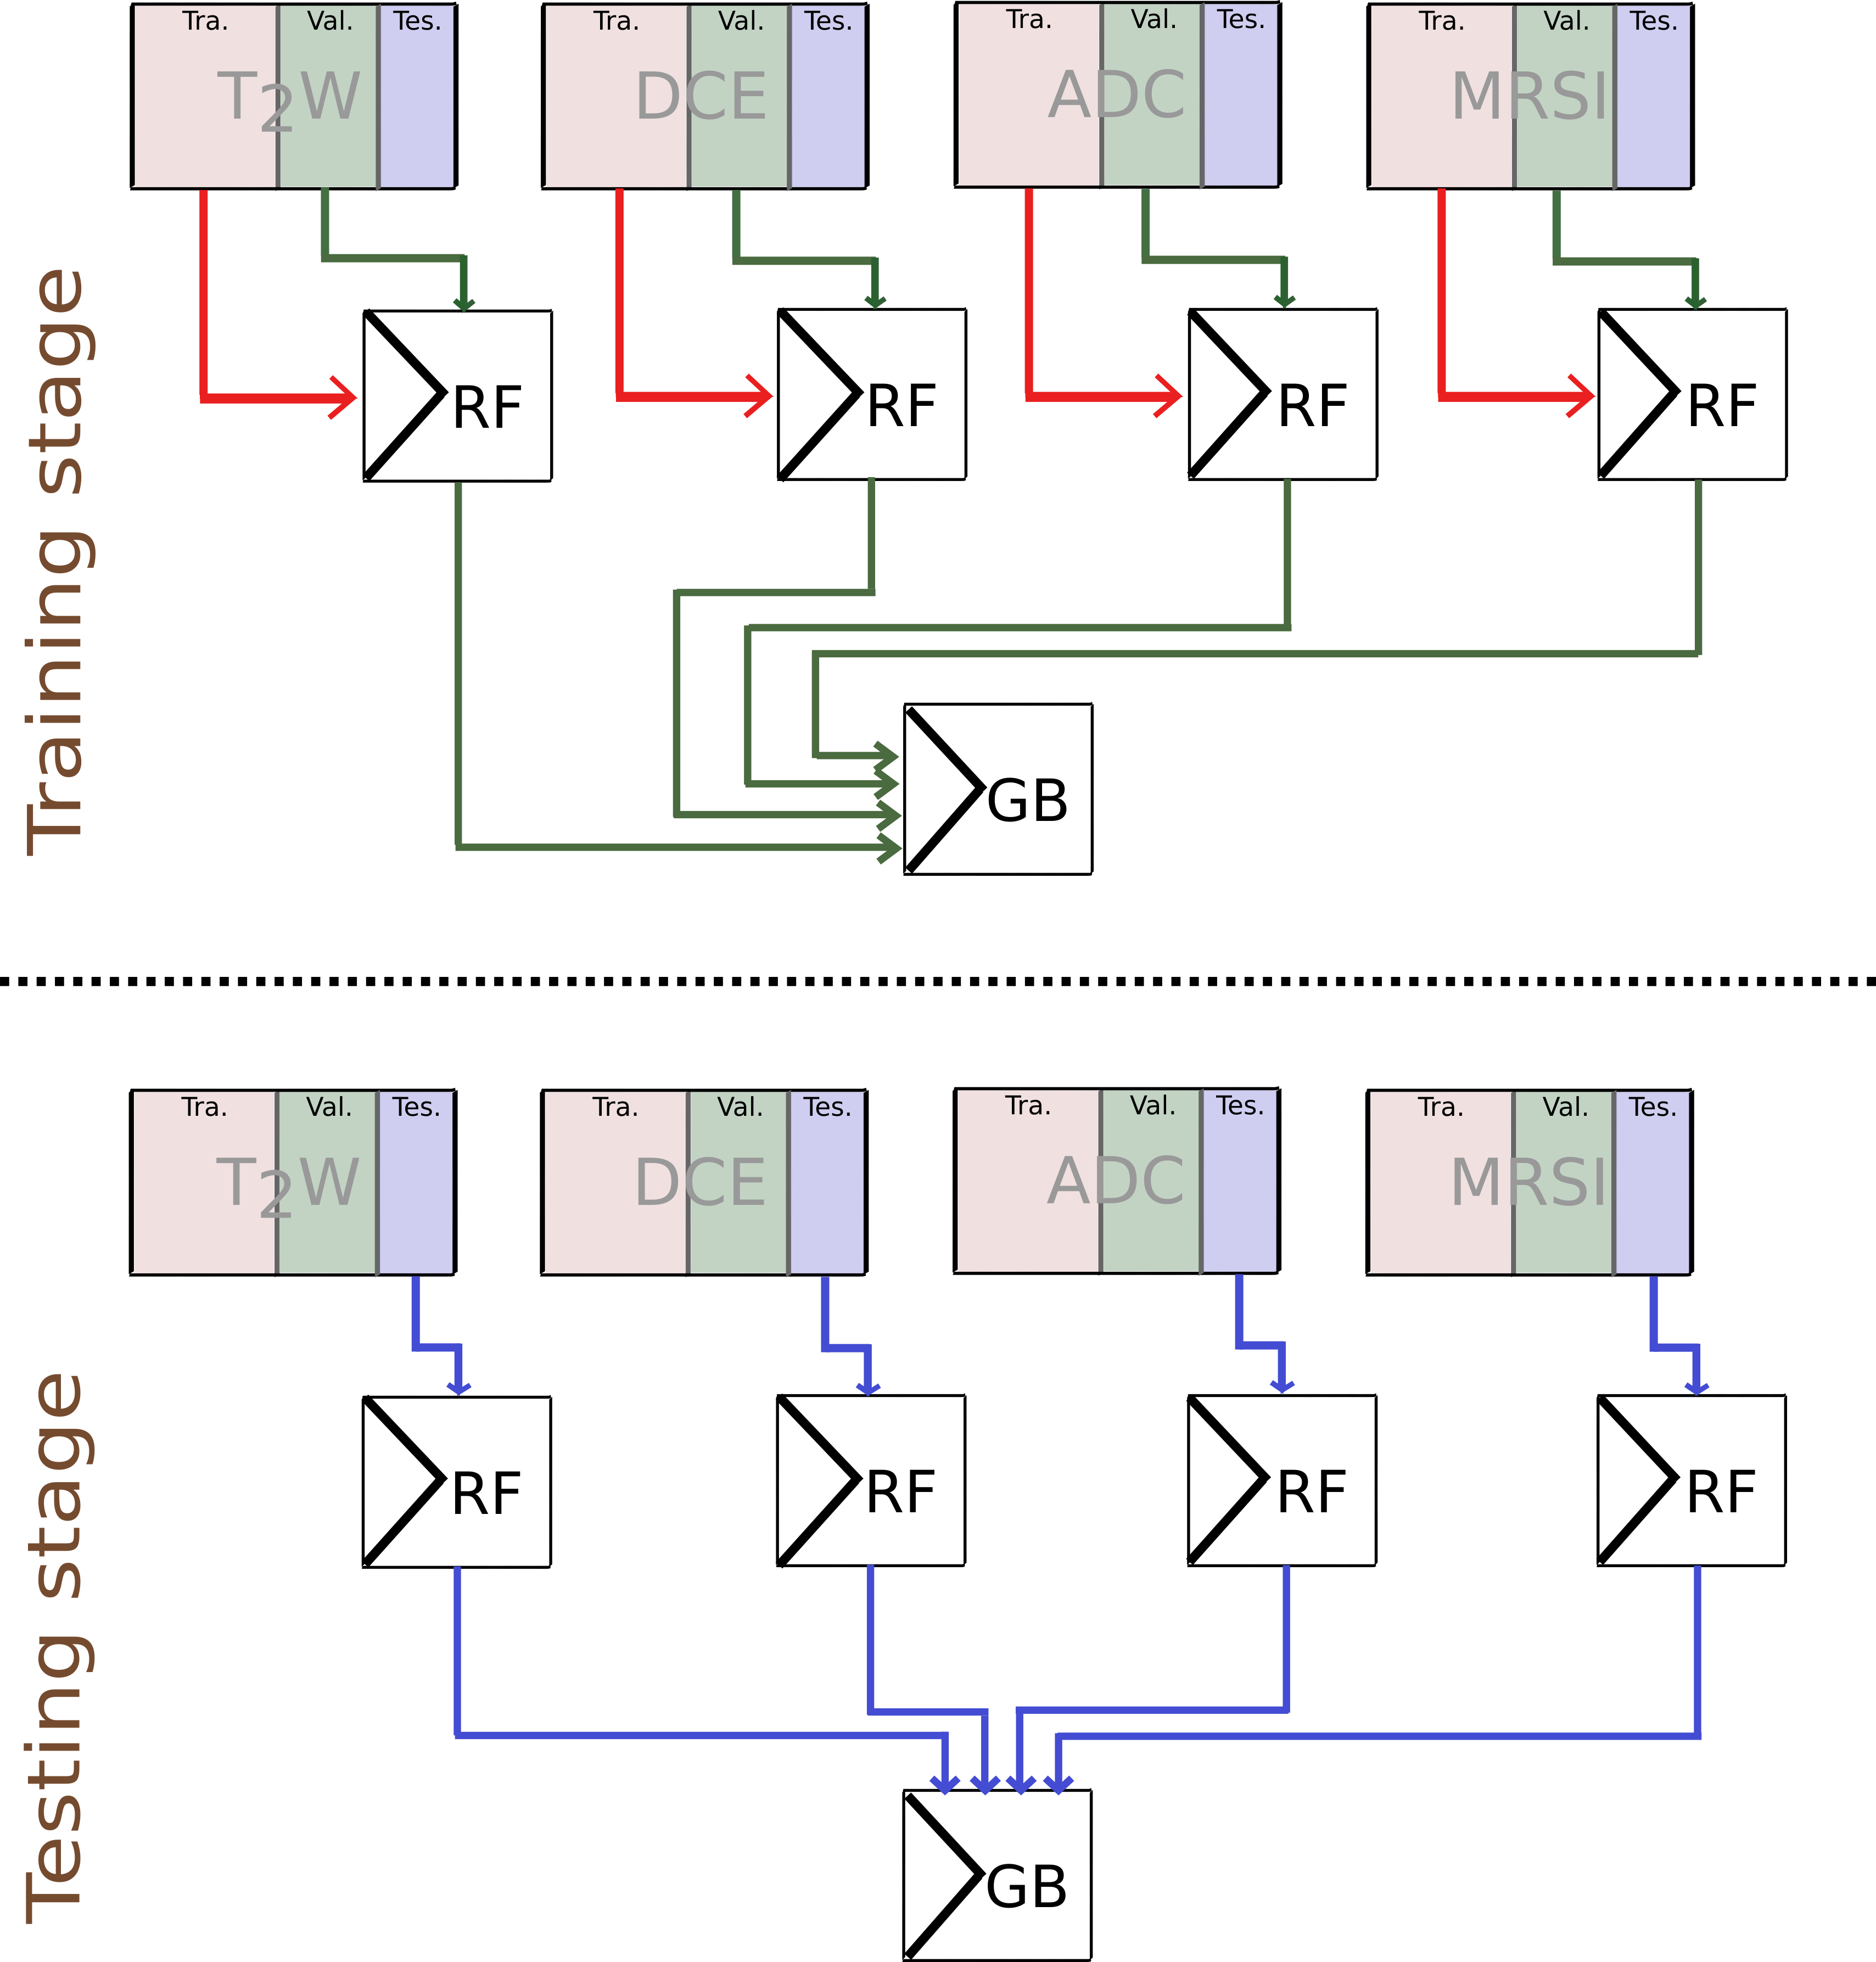
\includegraphics[width=0.5\linewidth]{content/figures/stacking_gb.png}
% %   \caption[The principle of stacking.]{The principle of stacking. First,
% %     training samples (red) are used to train each individual \ac{rf}.
% %     Subsequently, a validation set (green) is provided to each \ac{rf} which
% %     outputs a set of probabilities used for the classification of the
% %     meta-classifier. Finally, a test set is used to asses the classification
% %     performance to whole stack.}
% %   \label{fig:stacking}
% % \end{figure}

% Additionally, we use stacking to create ensemble of base learners using a meta-classifier~\cite{wolpert1992stacked}.
% \Acl{fig}~\ref{fig:stacking} illustrate the principle of stacking.
% Stacking consists in a two-stage learning:
% (i) First, a set of training samples is used to train each individual base learner and
% (ii) subsequently, a set of validation samples is provided to each \ac{rf} which individually output a corresponding set of probability used to train a meta-classifier.
% Finally, the stack of classifiers is assessed by providing a test set which is going through the base learners and the meta-classifier.

% In the later experiments, \ac{adb} and \ac{gb} are chosen as meta-classifiers to aggregate the base learners in the stacking strategies.
% The difference between \ac{adb} and \ac{gb} lie in the fact the this
% minimization procedure.

\section{Experiment and results}
\label{sec:experiments}

\Acl{sec}\,\ref{sec:experiments:mpmri-comparison} analyzes the impact of \ac{mpmri}, which
is summarized in \Ac{fig}\,\ref{fig:modality-combination} where the results from
individual modalities are compared to different strategies for combining the
information brought by each modality.
Whereas, \ac{sec}\,\ref{sec:experiments:light} discusses some particular aspects
of the workflow in \Ac{sec}\,\ref{sec:framework} in order to bring each
modality to its best light in order to compose \Ac{fig}\,\ref{fig:modality-combination:separeate_modalities}.

\subsection{\ac{cap}-\ac{cad} bits}
\label{sec:experiments:mpmri-comparison}
\paragraph{The value of supplying \ac{dce} data directly}
\paragraph{For the case of \ac{dce} data, a good normalization is all you need.}

The features derived from the \ac{dce} modality can be categorized in: 
(i) quantitative methods which describe the signal based on parameter values
better fitting a given pharmacokinetic model such as Toft or Brix;
(ii) semi-quantitative methods that use some descriptor such as wash in and wash
out to embed the signal;
or (iii) the entire signal.

% Despite literature favoring the first two groups of
% features~\cite{lemaitre2015computer} \emph{because they integrate over the
%   singal independently}, we argue that a proper normalization of
% the entire signal that brings \emph{all the patients, all the under the same
%   coordinate system} leads to better results. 
%
\Acl{fig}\,\ref{fig:DCE-norm} compares the quantitative and semi-quantitative
features against the entire \ac{dce} signal with (and without) normalization,
showing that properly normalized data brings the most discriminating information
from \ac{dce} modality, closely followed by the semi-quantitative approaches.
Based this results quantitative methods create the least discriminating space.

\begin{figure}
  \hspace*{\fill}
  \subfigure[Performance of the quantitative methods on \acs*{dce}.] {
    \includegraphics[width=.45\textwidth]
    {images/DCE-normalization/normalized_methods_0.pdf}
  }
  \hfill
  \subfigure[Performance of enhanced \acs*{dce} signal.]{
  \includegraphics[width=.45\textwidth]
  {images/DCE-normalization/full_signal_0.pdf}
  }
  \hspace*{\fill}
  \caption[DCE] {DCE}
  \label{fig:DCE-norm}
\end{figure}

% \subparagraph{\ac{mrsi} features}
% Due to unavailability of some unsuppressed water acquisition, absolute quantification as presented by \citeauthor{trigui2017automatic} could not be computed~\cite{trigui2017automatic}.
% Therefore, likewise in~\cite{Parfait2012}, three different techniques are used to extract discriminative features: (i) relative quantification based on metabolite quantification, (ii) relative quantification based on bounds integration, and (iii) spectra extraction.
% \subparagraph{Anatomical features}
% Beside the aforementioned features specific at each modality, anatomical features as proposed by \citeauthor{Chen2002} and \citeauthor{Litjens2014} are computed~\cite{Chen2002,Litjens2014}.
% Therefore, 4 different metrics are computed based on the relative distance to the prostate boundary as well as the prostate center, and the relative position in the Euclidean and cylindrical coordinate systems.

\section{The advantage of mpmri}%\ac{mpmri}}
\label{sec:experiments:mpmri-comparison}

As aforementioned, \ac{fig}\,\ref{fig:modality-combination} compares the best
results of each individual image modality (\ac{t2w}-\ac{mri}, \ac{dce}-\ac{mri},
\ac{adc} map and \ac{mrsi}) in 
\ac{fig}\,\ref{fig:modality-combination:separeate_modalities}) against three
different manners of combining them in \ac{fig}\,\ref{fig:modality-combination:combined}:
(i) in blue, a feature vector composed with the selected features of each image
modality (those selected to produce
\Ac{fig}\,\ref{fig:modality-combination:separeate_modalities}) is fitted to a
\ac{rf} classifier.
(ii) In green, the classifiers producing
\Ac{fig}\,\ref{fig:modality-combination:separeate_modalities} are used to train
a stacking classifier with a \ac{gb} as meta-classifier.
And (iii) in red, all the features from all modalities (see
\Ac{tab}\,\ref{tab:feat}) concatenated as a single vector are directly fitted to
a \ac{rf} classifier.

The best results are achieved using the last configuration with an \ac{auc} of
$0.836 \pm 0.083$.
\Acl{fig}\,\ref{fig:resultcad} illustrates qualitative results of this
configuration by overlapping the probability map of having a \ac{cap} with the
original \ac{t2w}-\ac{mri} slice, for 6 diverse patients.
\emph{Something more comparing to single modality plot.}

\begin{figure}
  \hspace*{\fill}
  \subfigure[] {
    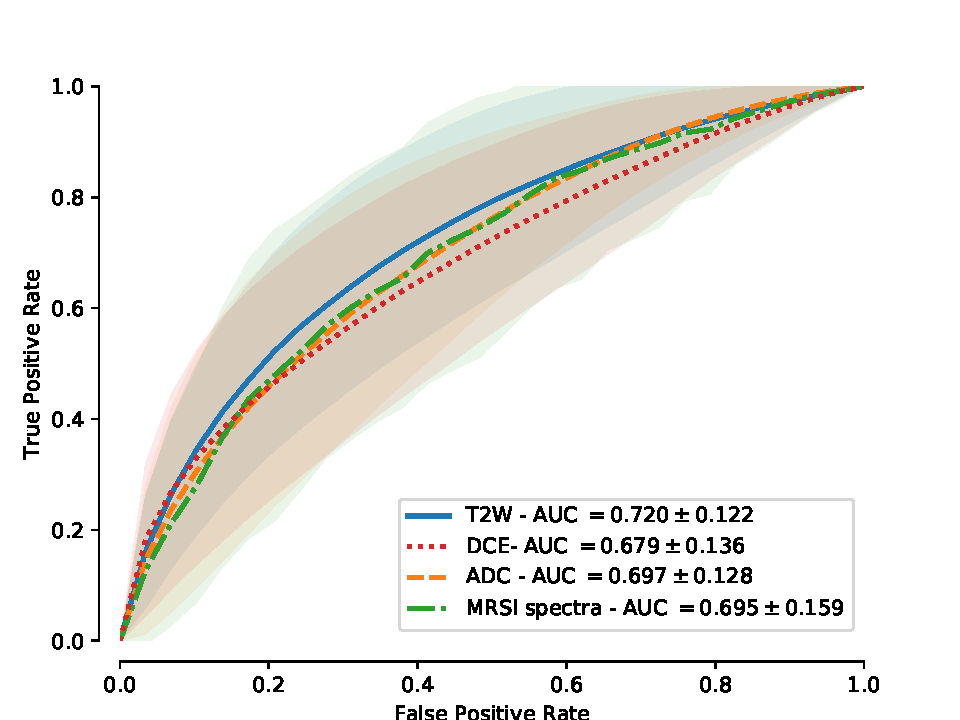
\includegraphics[width=.45\textwidth]
    {images/all.pdf}
    \label{fig:modality-combination:separeate_modalities}
  }
  \hfill
  \subfigure[Analysis of feature combination approaches after fine tuning.]{
    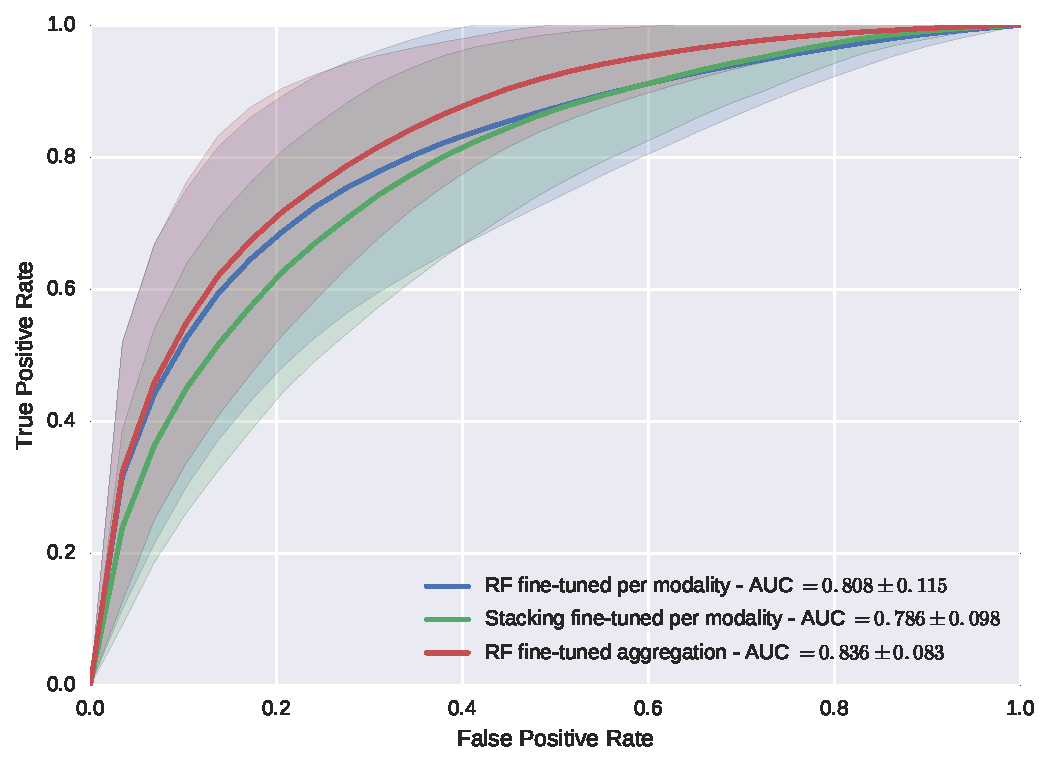
\includegraphics[width=.45\textwidth]
    {content/figures/exp-5/combine_all.pdf}
    \label{fig:modality-combination:combined}
  }
  \hspace*{\fill}
  \caption[modality combination] {Modality combination}
  \label{fig:modality-combination}
\end{figure}

Due to the limited body of work using \ac{mrsi} data in \ac{cap}-\ac{cad}
systems~\cite{lemaitre2015computer}, we also compare the stacking strategy with
and without \ac{mrsi} data in order to see its influence. We observe that with
no \ac{mrsi} data the final performance drops from 
$0.786 \pm 0.098$ to $0.756 \pm 0.092$.
This aligns with the fact that $29.2\%$ of the features selected when
concatenating all the features from all modalities are in fact from \ac{mrsi}
data (see \Ac{tab}\,\ref{tab:selfeatocc}).

\begin{figure}
  \hspace*{\fill}
  \subfigure[\acs{t2w}]{
    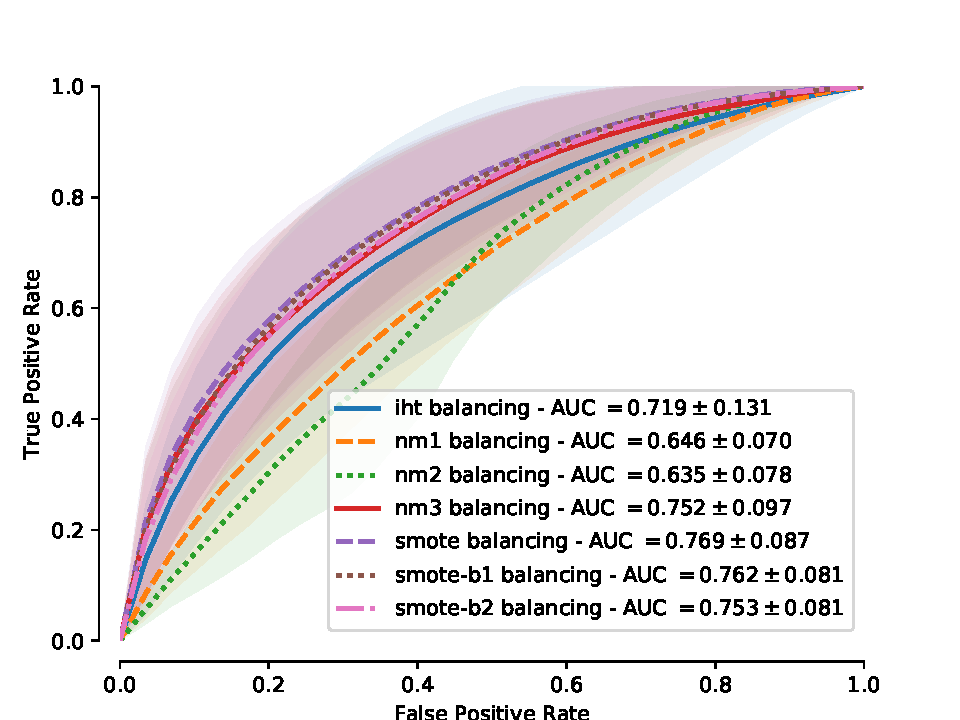
\includegraphics[width=.45\textwidth]
    {images/imbalance_effect/t2w.pdf}
  }
  \hfill
  \subfigure[\acs{adc}] {
    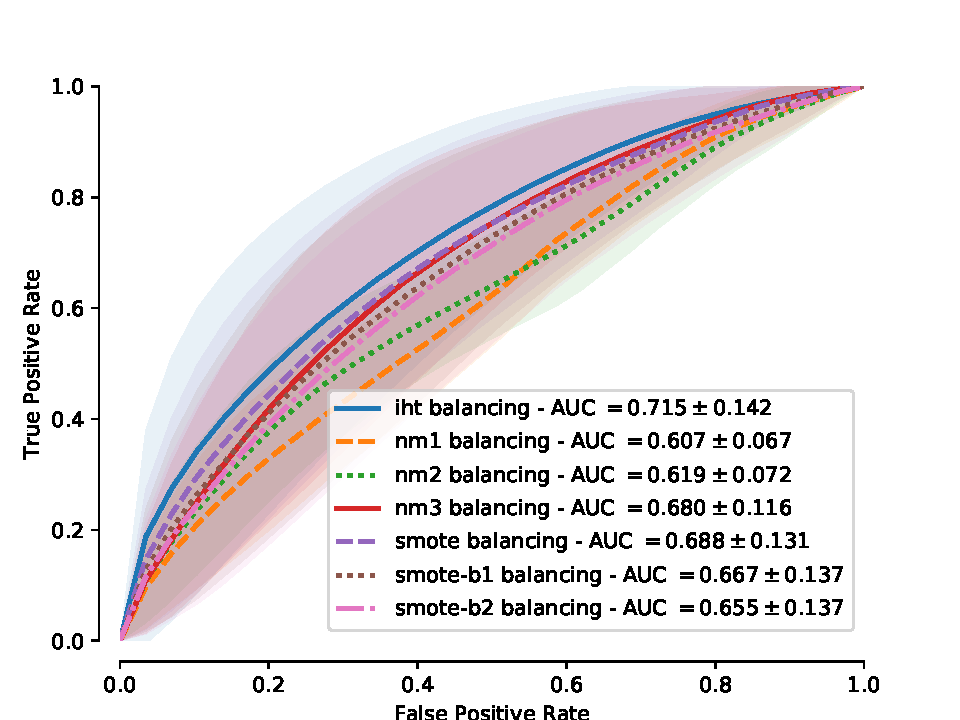
\includegraphics[width=.45\textwidth]
    {images/imbalance_effect/adc.pdf}
  }
  \hspace*{\fill}\\
  \hspace*{\fill}
  \subfigure[\acs{dce}] {
    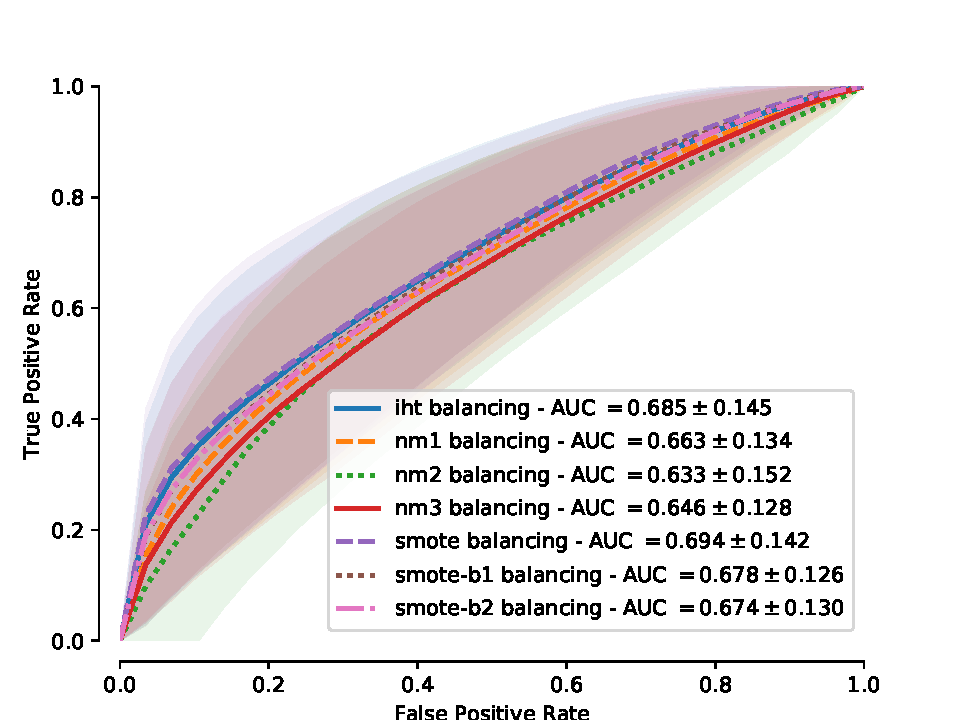
\includegraphics[width=.45\textwidth]
    {images/imbalance_effect/dce.pdf}
  }
  \hfill
  \subfigure[\acs{mrsi}]{
    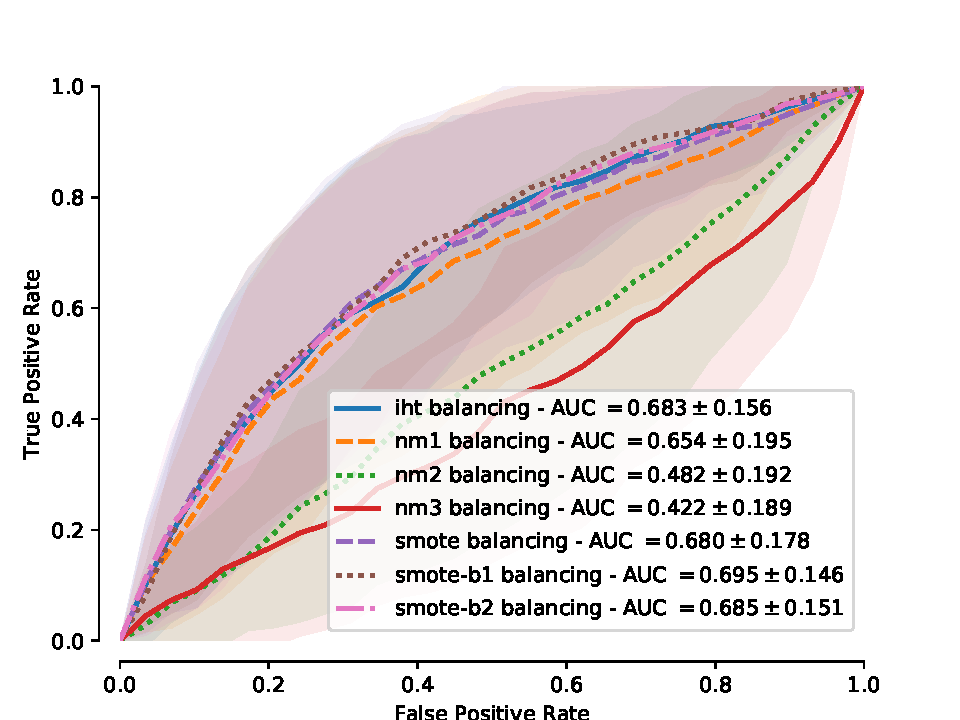
\includegraphics[width=.45\textwidth]
    {images/imbalance_effect/mrsi.pdf}
  }
  \hspace*{\fill}
  \caption[] {Imbalance effect}
  \label{fig:imbalance}
\end{figure}

\begin{figure}
  \hspace*{\fill}
  \subfigure[\acs{t2w} feature importance]{
    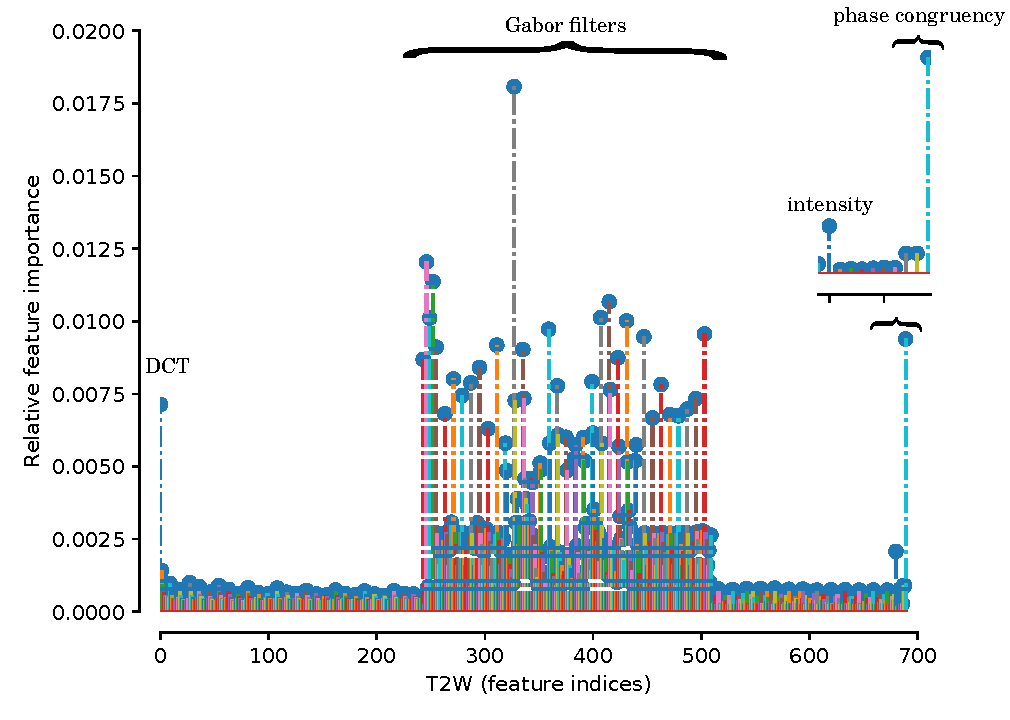
\includegraphics[width=.45\textwidth]
    {images/feature_importance/feature_importance_t2w_annotated.pdf}
  }
  \hfill
  \subfigure[\acs{adc} feature importance] {
    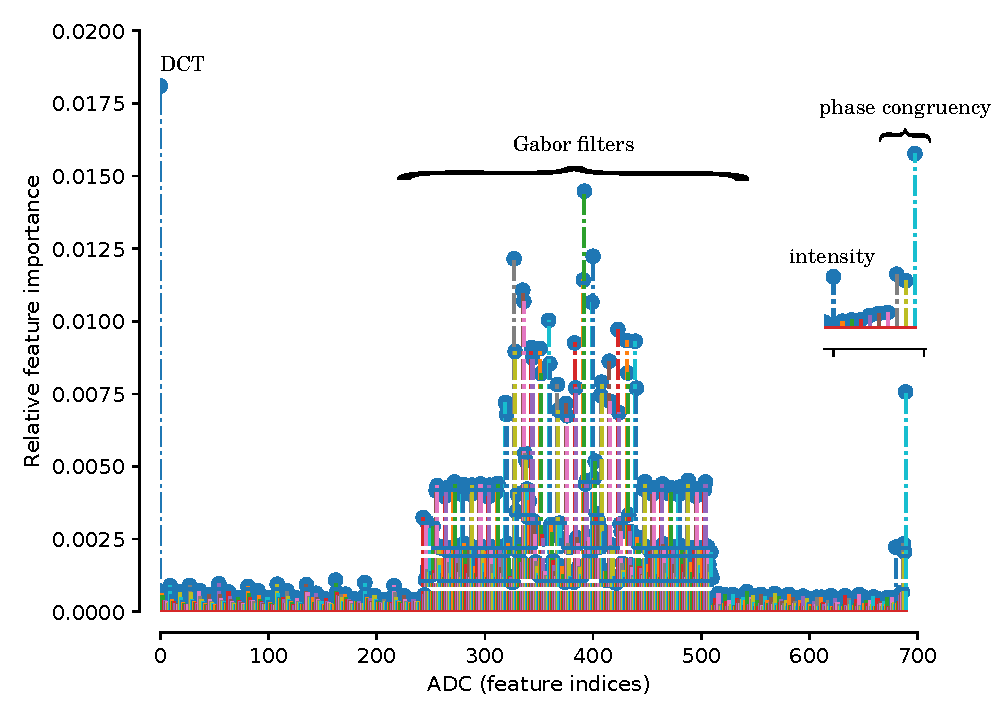
\includegraphics[width=.45\textwidth]
    {images/feature_importance/feature_importance_adc_annotated.pdf}
  }
  \hspace*{\fill}\\
  \hspace*{\fill}
  \subfigure[\acs{dce} feature importance] {
    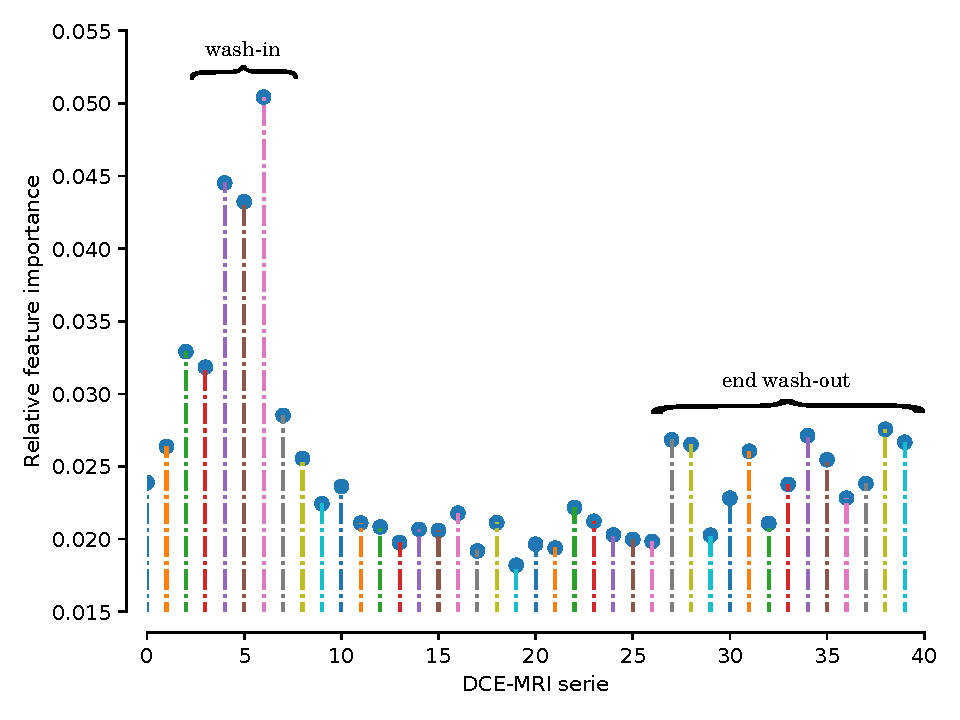
\includegraphics[width=.45\textwidth]
    {images/feature_importance/feature_importance_dce_annotated.pdf}
  }
  \hfill
  \subfigure[\acs{mrsi} feature importance]{
    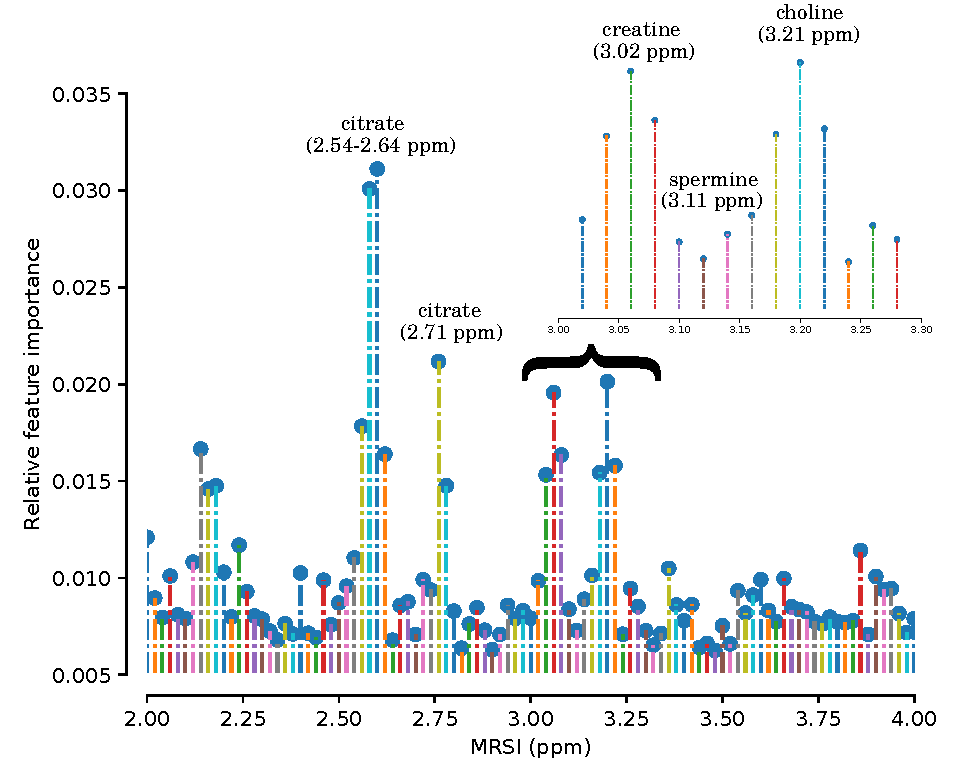
\includegraphics[width=.45\textwidth]
    {images/feature_importance/feature_importance_mrsi_annotated.pdf}
  }
  \hspace*{\fill}
  \caption[DCE] {Feature importance}
  \label{fig:feat_importance}
\end{figure}

\section{Conclusion}
\label{sec:conclusion}

% this review has presented an overview and classification of the research related
% to \ac{cad} development for \ac{cap} using multi-parametric \ac{mri} data. we
% aimed at providing background information regarding multi-parametric \ac{mri}
% imaging techniques and a description of the work-flow in the different \ac{cad}
% stages. the methods used in the literature for each of these stages have been
% reviewed along with the available results of the \ac{cad} systems. moreover,
% insight discussions and possible future research directions have also been
% given. finally, a multi-parametric multi-vendor dataset has been made available
% to the research community in order to provide a standardised platform for
% \ac{cad} development and evaluation for \ac{cap} using multi-parametric
% \ac{mri}.

% In this regard, \ac{mpmri} is frequently
% used to build robust \ac{cad} systems to detect, localize, and grade \ac{cap}.
% In general, \ac{cad} systems are based on \ac{mpmri} which potentially combines
% several of the following modalities~\citep{lemaitre2015computer}:
% \ac{t2w}-\ac{mri}, \ac{dce}-\ac{mri}, \ac{adc} maps, and \ac{mrsi}.

\begin{table}
  \caption{Selected feature and number of occurrence for \acs*{t2w}-\acs*{mri}, \acs*{adc} map, and one all the features are concatenated.}
  \centering
  \scriptsize
  \begin{tabular}{llllll}
    \toprule
    \multicolumn{1}{c}{\textbf{\acs*{t2w}-\acs*{mri}}} & \multicolumn{1}{c}{\textbf{\acs*{adc}}} & \multicolumn{1}{c}{\textbf{\acs*{t2w}-\acs*{mri}}} & \multicolumn{1}{c}{\textbf{\acs*{adc}}} & \multicolumn{1}{c}{\textbf{\acs*{dce}-\acs*{mri}}} & \multicolumn{1}{c}{\textbf{\acs*{mrsi}}} \\
    \cmidrule(lr){1-1} \cmidrule(lr){2-2} \cmidrule(lr){3-6}
    8 edges & 1 \acs*{dct} & 113 Gabor filters & 53 Gabor filters & 14 samples  & 78 samples \\
    155 Gabor filters & 32 Gabor filters & 1 phase congruency & 2 phase congruency & & \\ 
    2 Haralick features & 1 phase congruency & 4 edges & & & \\
    1 intensity & & 1 intensity & & & \\
    4 \acs*{lbp} & & & & & \\
    2 phase congruency & & & & & \\
    \cmidrule(lr){1-1} \cmidrule(lr){2-2} \cmidrule(lr){3-6}
    \multicolumn{1}{c}{\textbf{172 features}} & \multicolumn{1}{c}{\textbf{34 features}} & \multicolumn{4}{c}{\textbf{267 features}} \\
    \bottomrule
  \end{tabular}
  \label{tab:selfeatocc}
\end{table}


\begin{landscape}
\begin{figure}
  \hspace*{\fill}
  \subfigure[\acs*{auc} = 0.922]{\label{fig:pat634}\includegraphics[width=.45\textwidth]{images/qualitative_results/patient_634.pdf}}
  \hfill
  \subfigure[\acs*{auc} = 0.942]{\label{fig:pat778}\includegraphics[width=.45\textwidth]{images/qualitative_results/patient_778.pdf}}
  \hfill
  \subfigure[\acs*{auc} = 0.914]{\label{fig:pat1036}\includegraphics[width=.45\textwidth]{images/qualitative_results/patient_1036.pdf}}
  \hspace*{\fill}\\
  \hspace*{\fill}
  \subfigure[\acs*{auc} = 0.692]{\label{fig:pat634}\includegraphics[width=.45\textwidth]{images/qualitative_results/patient_410.pdf}}
  \hfill
  \subfigure[\acs*{auc} = 0.879]{\label{fig:pat778}\includegraphics[width=.45\textwidth]{images/qualitative_results/patient_784.pdf}}
  \hfill
  \subfigure[\acs*{auc} = 0.735]{\label{fig:pat1036}\includegraphics[width=.45\textwidth]{images/qualitative_results/patient_1041.pdf}}
  \hspace*{\fill}
  \caption[Illustration the resulting detection of our \acs*{mpmri} \acs*{cad} for \acs*{cap} detection.]{Illustration the resulting detection of our \acs*{mpmri} \acs*{cad} for \acs*{cap} detection. The blue contours corresponds to the \ac{cap} while the \texttt{jet} overlay represents the probability.}
  \label{fig:resultcad}
\end{figure}
\end{landscape}

% \acresetall
\section{Introduction}\label{chap:6}

In this chapter, we develop and investigate a \ac{cad} system for the \ac{cap} detection, using all \ac{mri} modalities, namely \ac{t2w}-\ac{mri}, \ac{dce}-\ac{mri}, \ac{dw}-\ac{mri}, and \ac{mrsi}.
Furthermore, we address some of the issues drawn in the conclusion of \acs{chp}\,\ref{chap:3}: (i) the methods investigated in \acs{chp}\,\ref{chap:5} are used in the pre-processing step of the proposed \ac{cad}; (ii) the discriminative power of each individual modality is investigated; (iii) the problem of learning from imbalanced dataset is investigated using state-of-the-art methods as well as (iv) several strategies for feature selection and combination.

Therefore, the organization of this chapter is as follows: the methodology is described in \acs{sec}\,\ref{sec:chp6:method} by presenting the image regularization framework as well as the image classification framework. \Acl{sec}~\ref{sec:chp6:exp-res} provides different experiments to investigate the performance of the proposed \ac{cad} system. This chapter is concluded by a concise discussion in \acs{sec}\,\ref{sec:chp6:discussion}.

\section{Methodology}\label{sec:chp6:method}

Our \ac{mpmri} \ac{cad} system consists of seven different steps: pre-processing, segmentation, registration, feature detection, balancing, feature selection/extraction, and finally classification.
%% It should be noted that \ac{cad} system designed deals with multiparametric \ac{mri} data. 

\subsection{Pre-processing}\label{subsec:chp6:method:PP}

\begin{figure}
  \hspace*{\fill}
  \subfigure[]{\label{fig:adcpdf1}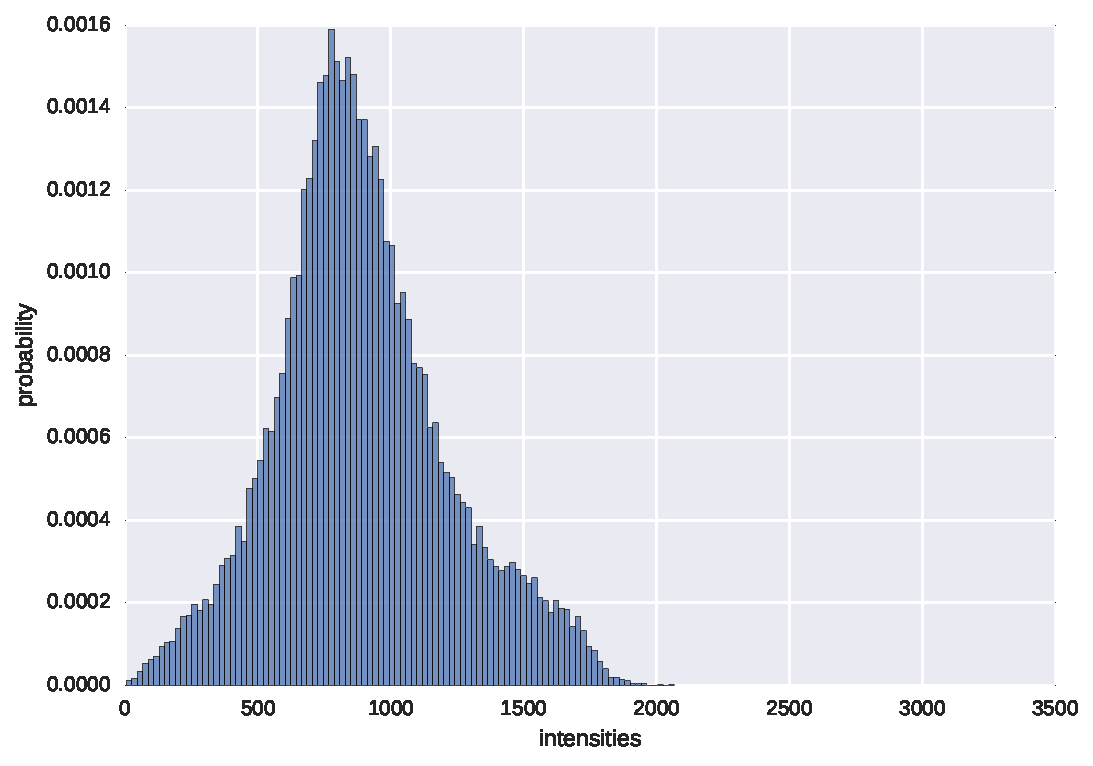
\includegraphics[width=.3\textwidth]{content/figures/adc_416.pdf}}
  \hfill
  \subfigure[]{\label{fig:adcpdf2}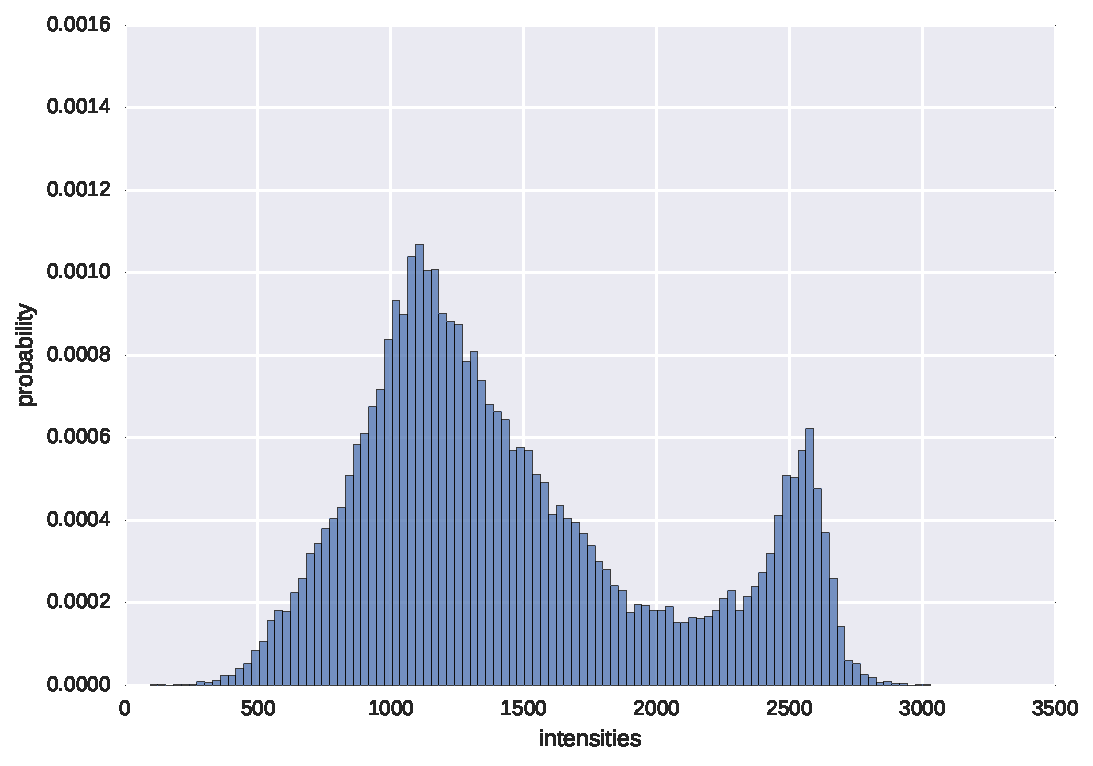
\includegraphics[width=.3\textwidth]{content/figures/adc_430.pdf}}
  \hfill
  \subfigure[]{\label{fig:adcpdf3}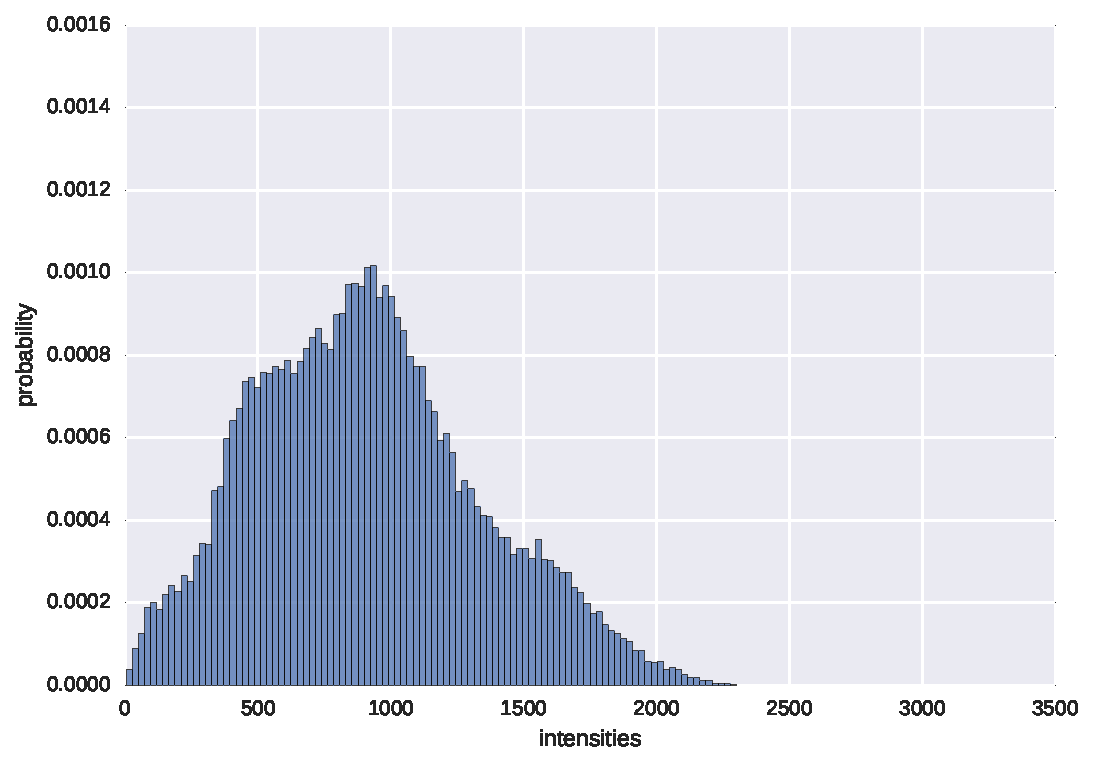
\includegraphics[width=.3\textwidth]{content/figures/adc_513.pdf}}
  \hspace*{\fill}
  \caption[Illustration of the \acs*{pdf} of the \acs*{adc} coefficients within the prostate.]{Illustration of the variability of the \acs*{pdf} of the \acs*{adc} coefficients within the prostate for 3 patients.}
  \label{fig:adcpdf}
\end{figure}


The reader can refer to \acs{sec}\,\ref{subsec:chp3img-reg:prepro} to have an extensive overview of the state-of-the-art methods used to pre-process \ac{mpmri} data.
Three types of pre-processing are used for \ac{mri} images: (i) noise filtering, (ii) bias correction, and (iii) standardization/normalization.
Our dataset is based on \SI{3}{\tesla} images without endorectal coil and therefore, the two first types of correction have not been considered as necessary.
Normalization is, however, a crucial step to reduce the inter-patient variations which allows to improve the learning during the classification stage.
\Ac{chp}~\ref{chap:5} presented two normalization methods to pre-process \ac{t2w}-\ac{mri} and \ac{dce}-\ac{mri}, respectively.
Therefore, we used these methods to standardize these images.
Regarding the \ac{adc} map normalization, the \ac{pdf} within the prostate does not follow a known distribution as depicted in \acs{fig}\,\ref{fig:adcpdf}.
Thus, one cannot use a parametric model to normalize these images and a non-parametric piecewise-linear normalization~\cite{Nyul2000} is the best option for this case.

Additionally, the \ac{mrsi} modality requires a specific pre-processing based on signal processing rather than image processing.
Therefore, the \ac{mrsi} modality has been pre-processed to correct the phase, baseline, and frequency.
Regarding the problem of phase correction and frequency alignment, we use the most efficient method of the state-of-the-art reviewed in \acs{sec}\,\ref{subsec:chp3img-reg:prepro}.
Indeed, as \citeauthor{Parfait2012} and \citeauthor{trigui2017automatic}~\cite{Parfait2012,trigui2016classification,trigui2017automatic}, the phase of each \ac{mrsi} spectra is corrected using the approach of \citeauthor{Chen2002}~\cite{Chen2002}.
Along the same line, the frequency shift of each spectra is corrected by aligning to \SI{4.65}{\ppm} the maximum of an inferred function fitted to the residuals of water, using a Voigt profile as in \acs{eq}\,\eqref{eq:voigt}.

\begin{equation}
  V(x; \sigma, \gamma) = \frac{\mathbf{R} \left[ w(z) \right]}{\sigma \sqrt{2\pi}} \ ,
  \label{eq:voigt}
\end{equation}

\noindent where $\mathbf{R} \left[ w(z) \right]$ is the real part of the Faddeva function for $z = \frac{x + i \gamma}{\sigma \sqrt{2}}$.

By assessing the qualitative results obtained in~\cite{Parfait2010}, the baseline correction method used by \citeauthor{Parfait2012} and \citeauthor{trigui2017automatic} does not provide an optimal solution for that matter.
The iterative low-pass filter enforces too much the smoothness of the baseline.
\citeauthor{xi2008baseline} proposed a baseline detection derived from a parametric smoothing model~\cite{xi2008baseline}.
The \ac{nmr} signal is formalized as a sum of a pure signal, the baseline function, and an additive Gaussian noise such as:

\begin{equation}
  y_i = b_i + \mu_i e^{n_i} + \varepsilon_i \ ,
  \label{eq:methodBaselineDetectionModel}
\end{equation}

\noindent where $y_i$ is the \ac{nmr} signal, $b_i$ is the baseline, $\mu_i$ is the true signal, and $n_i$ and $\varepsilon_i$ are Gaussian noises.

\citeauthor{xi2008baseline} propose to find the baseline function through an iterative optimization by maximizing the following cost function:

\begin{equation}
  F(b) = \sum_{i = 1}^{N} b_i - \frac{A^{*} N^4}{\sigma} \sum_{i = 1}^{N} (b_{i+1} + b_{i-1} - 2 b_i)^2 - \frac{1.25 B^{*}}{\sigma} \sum_{i = 1}^{N} (b_i - \gamma_i)^2 g(b_i - \gamma_i) \ ,
  \label{eq:methodBaselineDetectionCostFunction}
\end{equation}

\noindent where $g(b_i - \gamma_i)$ is the Heaviside function, $A^*$ and $B^*$ are the terms controlling the smoothness and negative penalties, respectively, $\sigma$ is an estimation of the standard deviation of the noise, and $N$ is the total number of points in the \ac{mrsi} signal.

The standard deviation of the noise $\sigma$ is estimated as in~\cite{xi2008baseline}, and the $A^{*}$ and $B^{*}$ are empirically set to $5 \times 10^{-6}$ and $100$, respectively, for all the \ac{mrsi} signal.
Setting these parameters allows to obtain an estimation of a smooth and possibly negative baseline, required by the aspect of the citrate peak in our \ac{mrsi} acquisition, as depicted in \acs{fig}\,\ref{fig:baselinemrsi}.

\begin{figure}
  \centering
  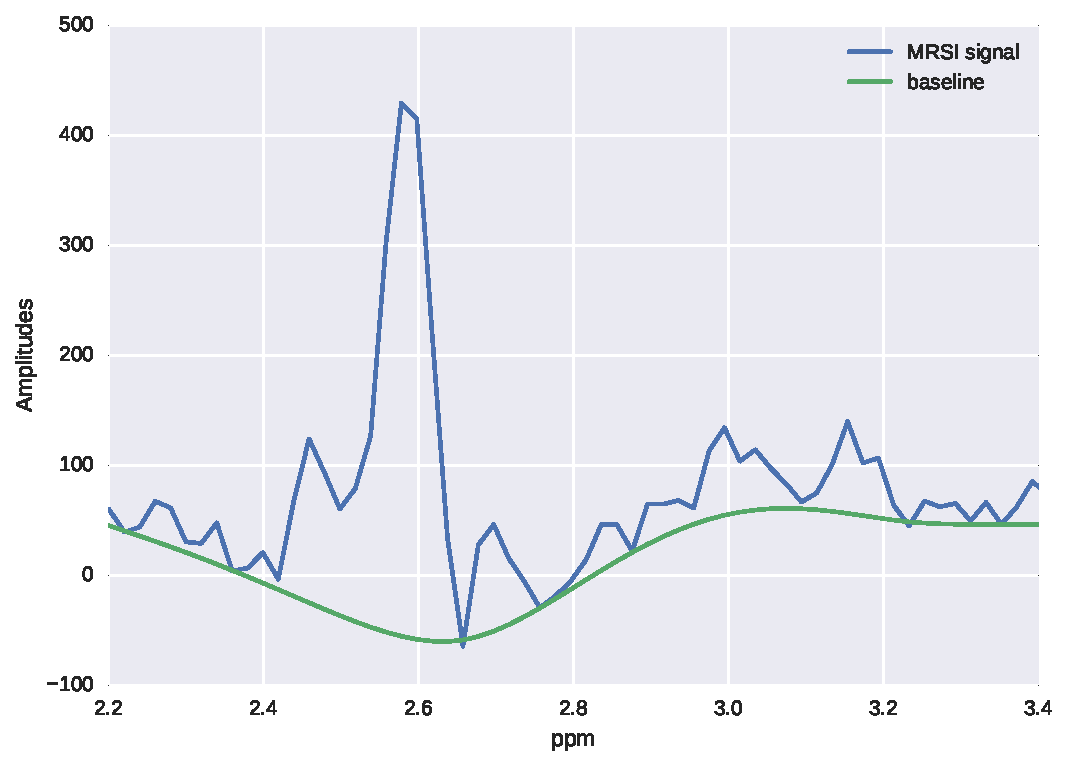
\includegraphics[width=0.5\linewidth]{content/figures/baseline_mrsi.pdf}
  \caption{Illustration of the detection of the baseline on an \acs*{mrsi} spectrum.}
  \label{fig:baselinemrsi}
\end{figure}

Additionally, each \ac{mrsi} spectrum is normalized using the L$_2$ norm, which has been shown to be the most efficient normalization method in \ac{mrsi} as discussed in \acs{sec}\,\ref{subsec:chp3img-reg:prepro}.

\subsection{Segmentation and registration}\label{subsec:chp6:method:Seg-Reg}

For this study, no segmentation method has been developed and the manual segmentation given by our radiologist has been used.
The prostate is suffering, however, from a misalignment between the different \ac{mri} modalities.
Therefore, three registrations have been developed to: (i) the patient motion during the \ac{dce}-\ac{mri} acquisition, (ii) the patient motion between the \ac{t2w}-\ac{mri} and the \ac{dce}-\ac{mri} acquisitions, and (iii) the patient motion between the \ac{t2w}-\ac{mri} and the \ac{adc} map acquisition.
All registrations are implemented in C++ using \ac{itk}.

The \ac{dce}-\ac{mri} acquisition being dynamic, some intra-patient motions might occur during the acquisition.
For each serie of this dynamic acquisition, each 3D volume is registered to the first volume acquired, to remove the residual motion.
The appearance in the \ac{dce}-\ac{mri} images, however, varies due to the presence or not of the contrast media.
Therefore, the metric chosen to be minimized is the \ac{mi} and the geometric transform has been set to a rigid transform.
The optimization is performed using a regular step gradient descent.

Once the intra-patient motions corrected, a registration to correct the alignment between the \ac{t2w}-\ac{mri} and the \ac{dce}-\ac{mri} acquisitions is performed.
For that matter, the prostate has been segmented in both modalities --- \ac{t2w}-\ac{mri} and \ac{dce}-\ac{mri} --- to create two binary masks.
Therefore, these 3D binary masks are directly registered using the \ac{mse} metric.
Unlike the previous registration, we use a more complex geometric transform by successively finding a rigid transformation, a coarse elastic transformation, and a fine elastic transformation.
B-splines transformation is used as the elastic transform.
These successive transformations allow to get a good initialization for the next transformation.
The transformation is inferred by minimizing the cost function using a regular step gradient descent.

The \ac{t2w}-\ac{mri} and \ac{adc} map acquisitions are registered using the same approach as for the registration of the \ac{t2w}-\ac{mri} and the \ac{dce}-\ac{mri} modalities.

Additionally, the \ac{cap}, \ac{pz}, and \ac{cg} are segmented on the \ac{t2w}-\ac{mri} and thus \ac{t2w}-\ac{mri} is used as the reference modality.

\subsection{Feature detection}\label{subsec:chp6:method:fea-det}

\begin{table}
  \caption{Features extracted in \acs*{t2w}-\acs*{mri} and \acs*{adc} volumes.}
  \centering
  \scriptsize
  \begin{tabularx}{\textwidth}{lXc}
    \toprule
    \textbf{Features} & \textbf{Parameters} & \textbf{\# dimensions} \\
    \midrule
    Intensity &  & 1 \\
    \acs*{dct} decomposition & window: \SI[product-units=repeat]{9x9x3}{\px} & 243 \\
    Kirsch filter &  & 2 \\
    Laplacian filter &  & 1 \\
    Prewitt filter &  & 3 \\
    Scharr filter &  & 3 \\
    Sobel filter &  & 3 \\
    Gabor filters & 4 frequencies $f \in [0.05, 0.25]$; 4 azimuth angles $\alpha \in [0, \pi]$; 8 elevation angles $\alpha \in [0, 2\pi]$ & 256 \\
    Phase congruency filter & 5 orientations; 6 scales & 3 \\
    Haralick filter & window: \SI[product-units=repeat]{9x9x3}{\px}; \# grey levels: 8; distance: \SI{1}{\px}; 13 directions & 169 \\
    \acs*{lbp} filter & 2 radii $r=\{1, 2\}$; 2 neighborhood sizes $N = \{8, 16\}$ & 6 \\
    \bottomrule
  \end{tabularx}
  \label{tab:featureadct2w}
\end{table}

To approach the task of automatic detection of \ac{cap} using machine learning, one has to extract a variety of feature specific to the \ac{mri} modality as presented in \acs*{sec}\,\ref{subsec:chp3:img-clas:CADX-fea-dec}.

\paragraph{\ac{t2w}-\ac{mri} and \ac{adc} map features}
Apart of using the normalized intensity, edge- and texture-based features are commonly extracted from \ac{t2w}-\ac{mri} and \ac{adc} map.
A set of common features earlier reported in \acs*{sec}\,\ref{subsec:chp3:img-clas:CADX-fea-dec} have been computed.
The following set of filters characterizing edges has been used: (i) Kirsch, (ii) Laplacian, (iii) Prewitt, (iv) Scharr, (v) Sobel, and (vi) Gabor.
Apart of Kirsch filter, the other filters are applied in 3D to get more information using a volume and not a slice, as it is usually done.
The extension of the most common edge detectors in 3D is obvious and will not be recalled.
However, 3D Gabor filters~\cite{wang2005face} are not commonly used and we recall their formulation in \acs*{eq}\,\eqref{eq:gabor3d}.

\begin{equation}
  g(\mathbf{x};\boldsymbol{\sigma},f,\theta,\phi) = \hat{g}(\mathbf{x};\boldsymbol{\sigma}) \exp(j 2 \pi f \left( x \sin \theta \cos \phi + y \sin \theta \sin \phi + z \cos \theta \right)) \ ,
  \label{eq:gabor3d}
\end{equation}

\noindent where,

\begin{equation}
  \hat{g}(\mathbf{x};\boldsymbol{\sigma}) = \frac{1}{{\left(2 \pi\right)}^{\frac{3}{2}}} \exp \left( -\frac{1}{2} \left( \frac{x^2}{\sigma_x^2} + \frac{y^2}{\sigma_y^2} + \frac{z^2}{\sigma_z^2} \right) \right) \ ,
  \label{eq:gabor3dgaussian}
\end{equation}

\noindent where $\mathbf{x}$ is the position vector $\{x,y,z\}$, $\boldsymbol{\sigma}$ is the standard deviation vector $\{\sigma_x,\sigma_y,\sigma_z\}$ of the 3D Gaussian envelope, $f$ is the radial center frequency of the sine wave, $\theta$ is the elevation angle, and $\phi$ is the azimuth angle.

Additionally, features based on phase congruency as proposed by \citeauthor{kovesi1999image} are computed~\cite{kovesi1999image}.
Therefore, from a set of Log-Gabor filter bank, the orientation image, the local weighted mean phase angle, and the phase angle are estimated at each voxel.

To characterize the local texture, both second-order \ac{glcm}-based features~\cite{Haralick1973} and rotation invariant and uniform \ac{lbp}~\cite{ojala2002multiresolution} are extracted.
To encode 3D information, the 13 first Haralick features --- refer to \acs{tab}~\ref{tab:glcm} --- are computed for the 13 possible directions.
For the same reason, the \ac{lbp} codes are computed for the three-orthogonal-planes of each \ac{mri} volume.

\Acl{tab}~\ref{tab:featureadct2w} summarizes the different features extracted with their corresponding parameters.
Note that all these features are extracted at each voxel of the volume.

\paragraph{\ac{dce}-\ac{mri} features} The extracted features for the \ac{dce}-\ac{mri} are exactly the ones describes in the previous chapter.
The reader can refer to \ac{sec}\,\ref{subsubsec:chp5:DCE-norm:stateart} for a detailed presentation of the different methods used.
In brief, the entire enhanced signal, semi-quantitative, and quantitative methods are computed. 

\begin{figure}
  \hspace*{\fill}
  \subfigure[]{\label{fig:goodfit}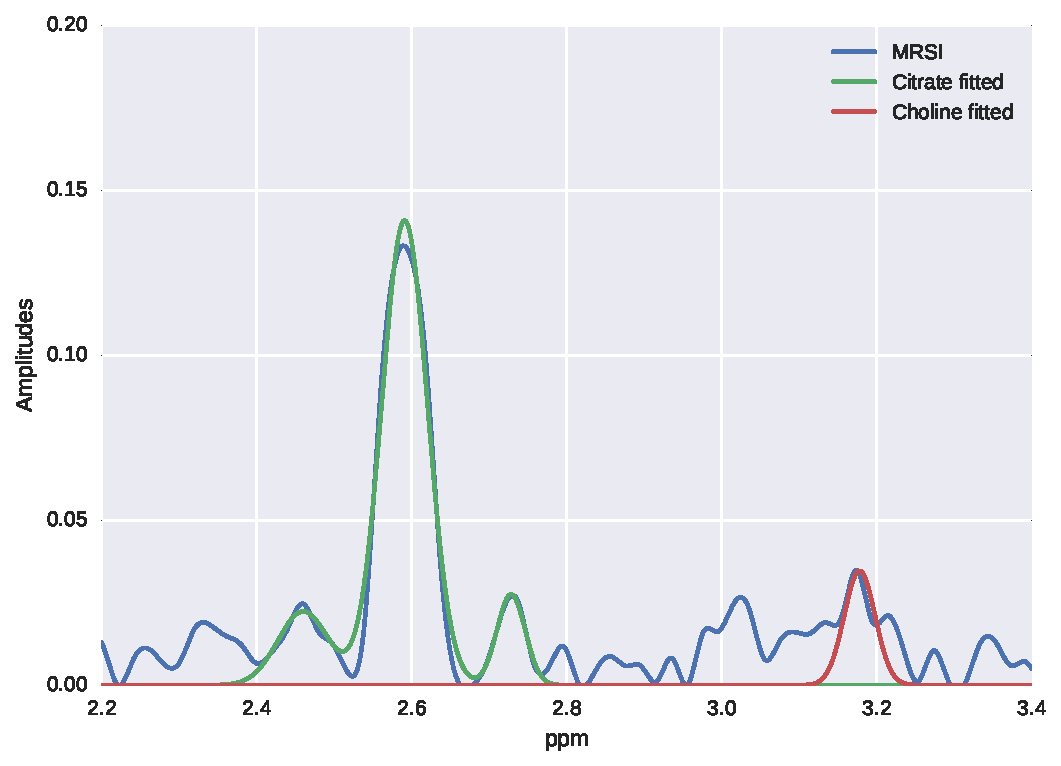
\includegraphics[width=.49\textwidth]{content/figures/meta_fitting.pdf}}
  \hfill
  \subfigure[]{\label{fig:wrongfit}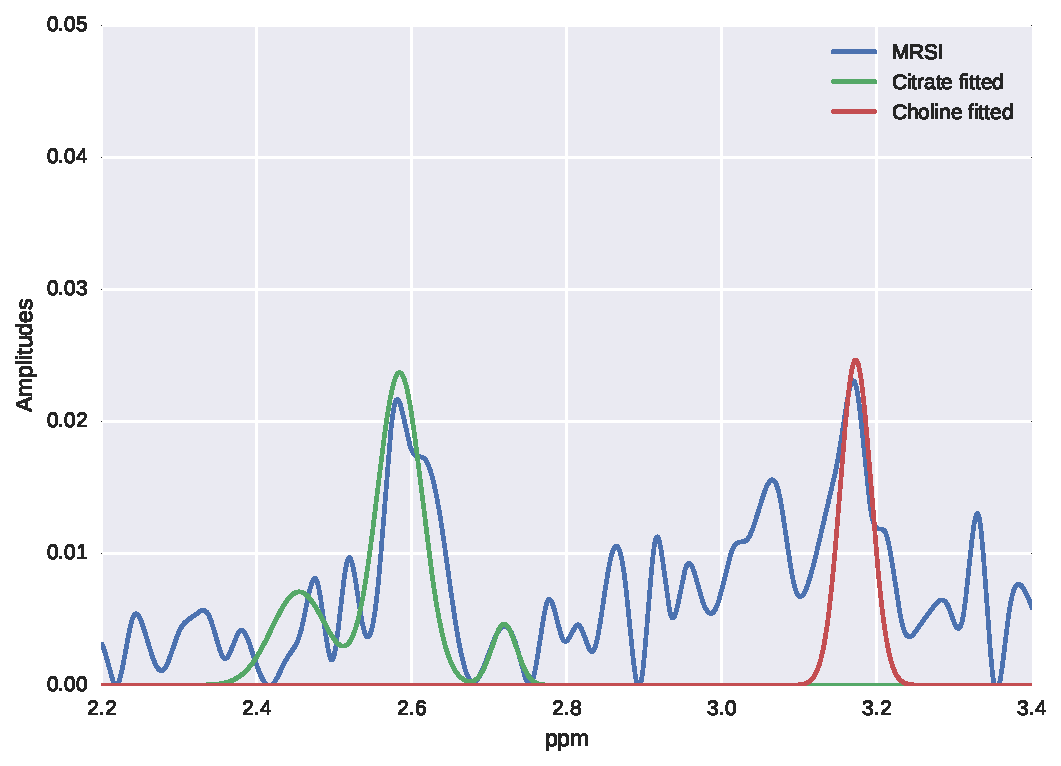
\includegraphics[width=.49\textwidth]{content/figures/meta_fitting_wrong.pdf}}
  \hspace*{\fill}
  \caption[Illustration of the metabolite fitting.]{Illustration of the metabolite fitting: \subref{fig:goodfit} the models are perfectly fitted for both citrate and choline; \subref{fig:wrongfit} the fitting of the citrate metabolite is inaccurate since it does not follow the \textit{a priori} model.}
  \label{fig:fitmeta}
\end{figure}

\paragraph{\ac{mrsi} features} \ac{mrsi}-based features have been explained in \acs{sec}\,\ref{subsubsec:chp3:img-clas:CADX-fea-dec:MRSI-fea}.
Due to unavailability of some unsuppressed water acquisition, absolute quantification as presented by \citeauthor{trigui2017automatic} could not be computed~\cite{trigui2017automatic}.
Therefore, likewise in~\cite{Parfait2012}, three different techniques are used to extract discriminative features: (i) relative quantification based on metabolite quantification, (ii) relative quantification based on bounds integration, and (iii) spectra extraction.

Relative quantification based on metabolite quantification relies on a robust integration of the citrate and choline signal based on peak modelling.
Therefore, we propose to tackle this problem as a non-linear least squares optimization problem by (i) quantifying the citrate peaks as a Gaussian mixture and (ii) quantifying the choline as a single Gaussian.

As illustrated in \acs{fig}\,\ref{fig:goodfit}, the \ac{mrsi} sequence imply a 3-peaks citrate metabolite.
Therefore, we propose the following model to represent our function as in \acs{eq}\,\eqref{eq:costcit}.

\begin{equation}
  M_1(x; \mathbf{w}) = \alpha_1 \mathcal{N}(x; \mu, \sigma_1) + \alpha_2 \mathcal{N}(x; \mu + \delta_2, \sigma_2) + \alpha_3 \mathcal{N(x; \mu - \delta_3, \sigma_3)} \ ,
  \label{eq:costcit}
\end{equation}

\noindent where $\mathcal{N}(\cdot)$ is a Gaussian distribution, $\mu$ is the central mean of the citrate, $\delta_2$ and $\delta_3$ are the shifts from the citrate central peak to the citrate side peaks, $\{\alpha_1, \alpha_2, \alpha_3\}$ are the amplitude factors of each Gaussian distribution, and $\{\sigma_1, \sigma_2, \sigma_3\}$ are the standard deviations of each Gaussian distribution. Additionally, we defined $\mathbf{w}$ as the vector containing the free parameters.

\Acl{eq}~\eqref{eq:costcit} is minimized under constraints as in \acs{eq}\,\eqref{eq:mincostcit}.


\begin{equation}
\begin{aligned}
& \argmin_{\mathbf{w}} 
& & | S(x) - M_1(x; \mathbf{w}) |^{2} \ , \label{eq:mincostcit} \\
& \text{subject to}
& & 2.54 < \mu < 2.68 \ , \\
&&& 0.06 < \delta_1, \delta_2 < 0.16 \ , \\
&&& 0.01 < \sigma_1, \sigma_2, \sigma_3 < 0.1 \ , \\
&&& \alpha_1, \alpha_2, \alpha_3 > 0 \ ,
\end{aligned}
\end{equation}

\noindent where $S(x)$ is the \ac{mrsi} signal. The different constraints are empirically set but based on the \emph{a priori} location of the peaks.

\Acl{fig}~\ref{fig:fitmeta} illustrates two fitting cases.
If the \ac{mrsi} signal follows the assumption regarding the model, which is generally the case --- i.e., a mixture of 3 Gaussian distributions ---, the signal is perfectly fitted as shown in \acs{fig}\,\ref{fig:goodfit}.
However, if the \ac{mrsi} signal does not obey to the model, the signal is fitted inaccurately as depicted in \acs{fig}\,\ref{fig:wrongfit}.

Theoretically, one could suggest to fit a Voigt mixtures instead of a Gaussian mixtures due to the presence of noise during the acquisition.
However, the use of Gaussian distributions reduces the number of parameters to be optimized and allows for a more robust optimization due to less interdependence between the bounds.

The choline metabolite is quantified on a similar manner assuming that there is only a single Gaussian distribution rather than a mixture.
Therefore the problem is formulated as:

\begin{equation}
  M_2(x; \mu, \sigma) = \alpha \mathcal{N}(x; \mu, \sigma) \ ,
  \label{eq:costcho}
\end{equation}

\noindent where $\mathcal{N}(\cdot)$ is a Gaussian distribution, $\mu$ is the center of the choline, $alpha$ is the amplitude factor, and $\sigma$ is the standard deviation. The optimization is performed such as:

\begin{equation}
\begin{aligned}
& \argmin_{\mathbf{\mu, \sigma}} 
& & | S(x) - M_2(x; \mu, \sigma) |^{2} \ , \label{eq:mincostcho} \\
& \text{subject to}
& & 3.17 < \mu < 3.21 \ , \\
&&& 0.001 < \sigma < 0.02 \ , \\
&&& \alpha > 0 \ .
\end{aligned}
\end{equation}

Finally, the citrate and choline fitted function are integrated to obtain the relative concentration of each metabolite.
Additionally, the ratio of the citrate over the choline is also computed.

A second solution to compute the relative concentration of each metabolite is proposed for the sake of comparison.
For both the choline and citrate, a local maximum is found near of the theoretical position of the peak.
Subsequently, a range is defined around each peak ---i.e., \SI{0.36}{\ppm} for the citrate and \SI{0.08}{\ppm} for the choline --- and the integral of the signal is computed using the Simpson's rule.

The third and last option corresponds on a cropping of the \ac{mrsi} signal from \SIrange{2}{4}{\ppm} as proposed in~\cite{Parfait2012}.

\paragraph{Anatomical features}

Beside the aforementioned features specific at each modality, anatomical features as proposed by \citeauthor{Chen2002} and \citeauthor{Litjens2014} are computed~\cite{Chen2002,Litjens2014}.
Therefore, 4 different metrics are computed based on the relative distance to the prostate boundary as well as the prostate center, and the relative position in the Euclidean and cylindrical coordinate systems.

\subsection{Feature balancing}\label{subsec:chp6:method:fea-bal}
Data imbalanced is a recurrent issue in classification, notably in medical data.
The problem of imbalanced dataset lies in the fact that one of the class has a smallest number of data --- i.e., in medical data, the class corresponding to patients with a disease --- compared with the other classes.
Therefore, solving the problem of imbalanced is equivalent to under- or over-sampling part of the dataset to obtain equal number of samples in the different classes.
In this section, several methods which will be used in the experiments are presented.

\subsubsection{\Acl*{us1}}
Techniques that reduce the number of samples of the majority class to be equal to the number of samples of minority class are referred to as \ac{us1} techniques.
%Considering the problem of imbalanced, \ac{us} is performed such that the number of samples of the majority class is reduced to be equal to the number of samples of the minority class.

\begin{description}
  \item[\Ac{nm}] offers three different methods to under-sample the majority class~\cite{mani2003knn}.
In \ac{nm1}, samples from the majority class are selected such that for each sample, the average distance to the $k$ \ac{nn} samples from the minority class is minimum.
\ac{nm2} diverges from \ac{nm1} by considering the $k$ farthest neighbours samples from the minority class.
In \ac{nm3}, a subset $M$ containing samples from the majority class is generated by finding the $m$ \ac{nn} from each sample of the minority class.
Then, samples from the subset $M$ are selected such that for each sample, the average distance to the $k$ \ac{nn} samples from the minority class is maximum.
In our experiment, $k$ and $m$ are fixed to 3.
\item[\Ac{iht}] select samples with a high hardness threshold~\cite{smith2014instance}.
Hardness indicates the likelihood of mis-classification rate for each samples.
The notation of instance hardness are drawn through the decomposition of $p(h \vert t)$ using Bayes' theorem, where $h$ represent the mapping function used to map input features to their corresponding labels and $t$ represents the training set.
\begin{equation}
  IH_h(\langle x_{i}, y_{i}\rangle) = 1 - p(y_i \vert x_i, h).\
\label{eq:iht}
\end{equation}
Therefore, under-sampling is performed by keeping the most probable samples --- i.e, filtering the samples with high hardness value --- through \ac{kcv} training sets while considering specific threshold for filtering.
%% The hardness of an instance is depedent on the instances in the training data and the algorithm used to produced h (h is a function mapping input features to their corresponding label , i.e, the classifier, or base learner function).

 
\end{description}

\subsubsection{\Acl*{os}}
In contrast to \ac{us1} techniques, data can be balanced by \ac{os} in which the new samples belonging to the minority class are generated, aiming at equalizing the number of samples in both classes.

\begin{description}
\item[\Ac{smote}] is a method to generate new synthetic samples~\cite{chawla2002smote}.
Let define $x_i$ as a sample belonging to the minority class.
Let define $x_{nn}$ as a randomly selected sample from the $k$-\ac{nn} of $x_i$, with $k$ set to 3.
A new sample $x_j$ is generated such that $x_j = x_i + \sigma \left( x_{nn} - x_i \right)$, where $\sigma$ is a random number in the interval $\left[0,1\right]$.
\item[\Ac{smoteb1}] over-samples the minority class samples similarly to \ac{smote}~\cite{han2005borderline}.
However, instead of using all the minority samples, it focuses on the borderline samples of minority class.
Borderline samples simply indicate the samples that are closer to the other class.
First, the borderline samples of minority class are detected.
A sample $x_{i}$ belongs to borderline samples if more than half of its $k$-\ac{nn} samples belong to the majority class.
Synthetic data is then created based on \ac{smote} method for borderline samples, by selecting 
Then, $s$-\ac{nn} of the minority class are selected to generate synthetic sample similarly to \ac{smote}.
 
\item[\Ac{smoteb2}] performs similarly to \ac{smoteb1}~\cite{han2005borderline}.
However, the $s$-\ac{nn} are not computed by only considering the minority class but by considering both classes.
The same generation rules as \ac{smote} is used.
\end{description}

\subsection{Feature selection and extraction}\label{subsec:chp6:method:fea-sel}

Feature selection and extraction are used in the experiment: (i) signal-based data --- i.e., \ac{mrsi} and \ac{dce}-\ac{mri} --- are decomposed using feature extraction methods while (ii) image-based features are selected through different feature selection methods.
These methods have been presented in \acs{sec}\,\ref{subsec:chp3:img-clas:CADX-fea-ext}.

Among those, \ac{pca}, sparse-\ac{pca}, and \ac{ica} are used to decompose signal-based data.

Similarly to \ac{pca} decomposition, \ac{ica} is projecting data on independent components~\cite{comon1994independent}.
However, it does not require orthogonality of the space and does not assume Gaussian distribution for each independent source.
Therefore, opposite to \ac{pca} it can recover uniquely the signals themselves rather than linear subspace in which the signals lie~\cite{murphy2012machine}.

Sparse-\ac{pca} is another approach for feature extraction and dimension reduction~\cite{zou2006sparse}.
Similarly to \ac{pca}, this approach projects the data as a linear combination of input data.
However, instead of using original data, it uses a sparse representation of the data, and therefore projects them as linear combination of few input components rather than all of them.
Referring to \acs{eq}\,\eqref{eq:eigpca}, the cost function of sparse-\ac{pca} is formulated to maximize the variance while maintaining the sparsity constraint:

\begin{eqnarray}
 && \argmax \quad   \mathbf{v}^{-1} \Sigma \mathbf{v}\ , \label{eq:sparsepca}\\ 
 && \text{subject to }  \Vert \mathbf{v} \Vert_{2} = 1\ , \nonumber \\
 && \Vert \mathbf{v} \Vert_{0} \leq k\ . \nonumber
\end{eqnarray}
\noindent where $k$ indicates that number of non-zero elements in $\mathbf{v}$.

Additionally to feature extraction, we use two methods of feature selection during the experiments.
The first feature selection is the one-way \ac{anova} test.
This test is based on computing the F-test which is the ratio of the between-group variability over the with-in group variability.
The F-value is computed for each pair of features and the $K$ feature dimensions corresponding to the largest F-values are kept.

Apart of using \ac{rf} as our main classifier, \ac{rf} provide information regarding the importance of each feature.
The feature importance in \ac{rf} is linked with the Gini importance.
In a tree classifier, the Gini impurity criterion of the child nodes is inferior to the parent node.
For each individual feature, adding the decrease of the Gini impurity along the tree gives information about the feature importance: the higher, the better.
Therefore, one can add the decrease of the Gini impurity across all the trees of a forest and obtain the importance of a specific feature for this forest.
Subsequently, the $K$ most important features are selected to perform the feature selection.

\subsection{Classification}\label{subsec:chp6:method:clas}
Variety of classifiers have been explained in \acs{sec}\,\ref{subsec:chp3:img-clas:CADX-clas}. 

Among those, \ac{rf} showed its reliability to lead to high classification performance.
That is why, \ac{rf} has been chosen as our base classifier --- allowing for feature selection as well --- to perform classification of individual modality as well as the combination of modalities.

\begin{figure}
  \centering
  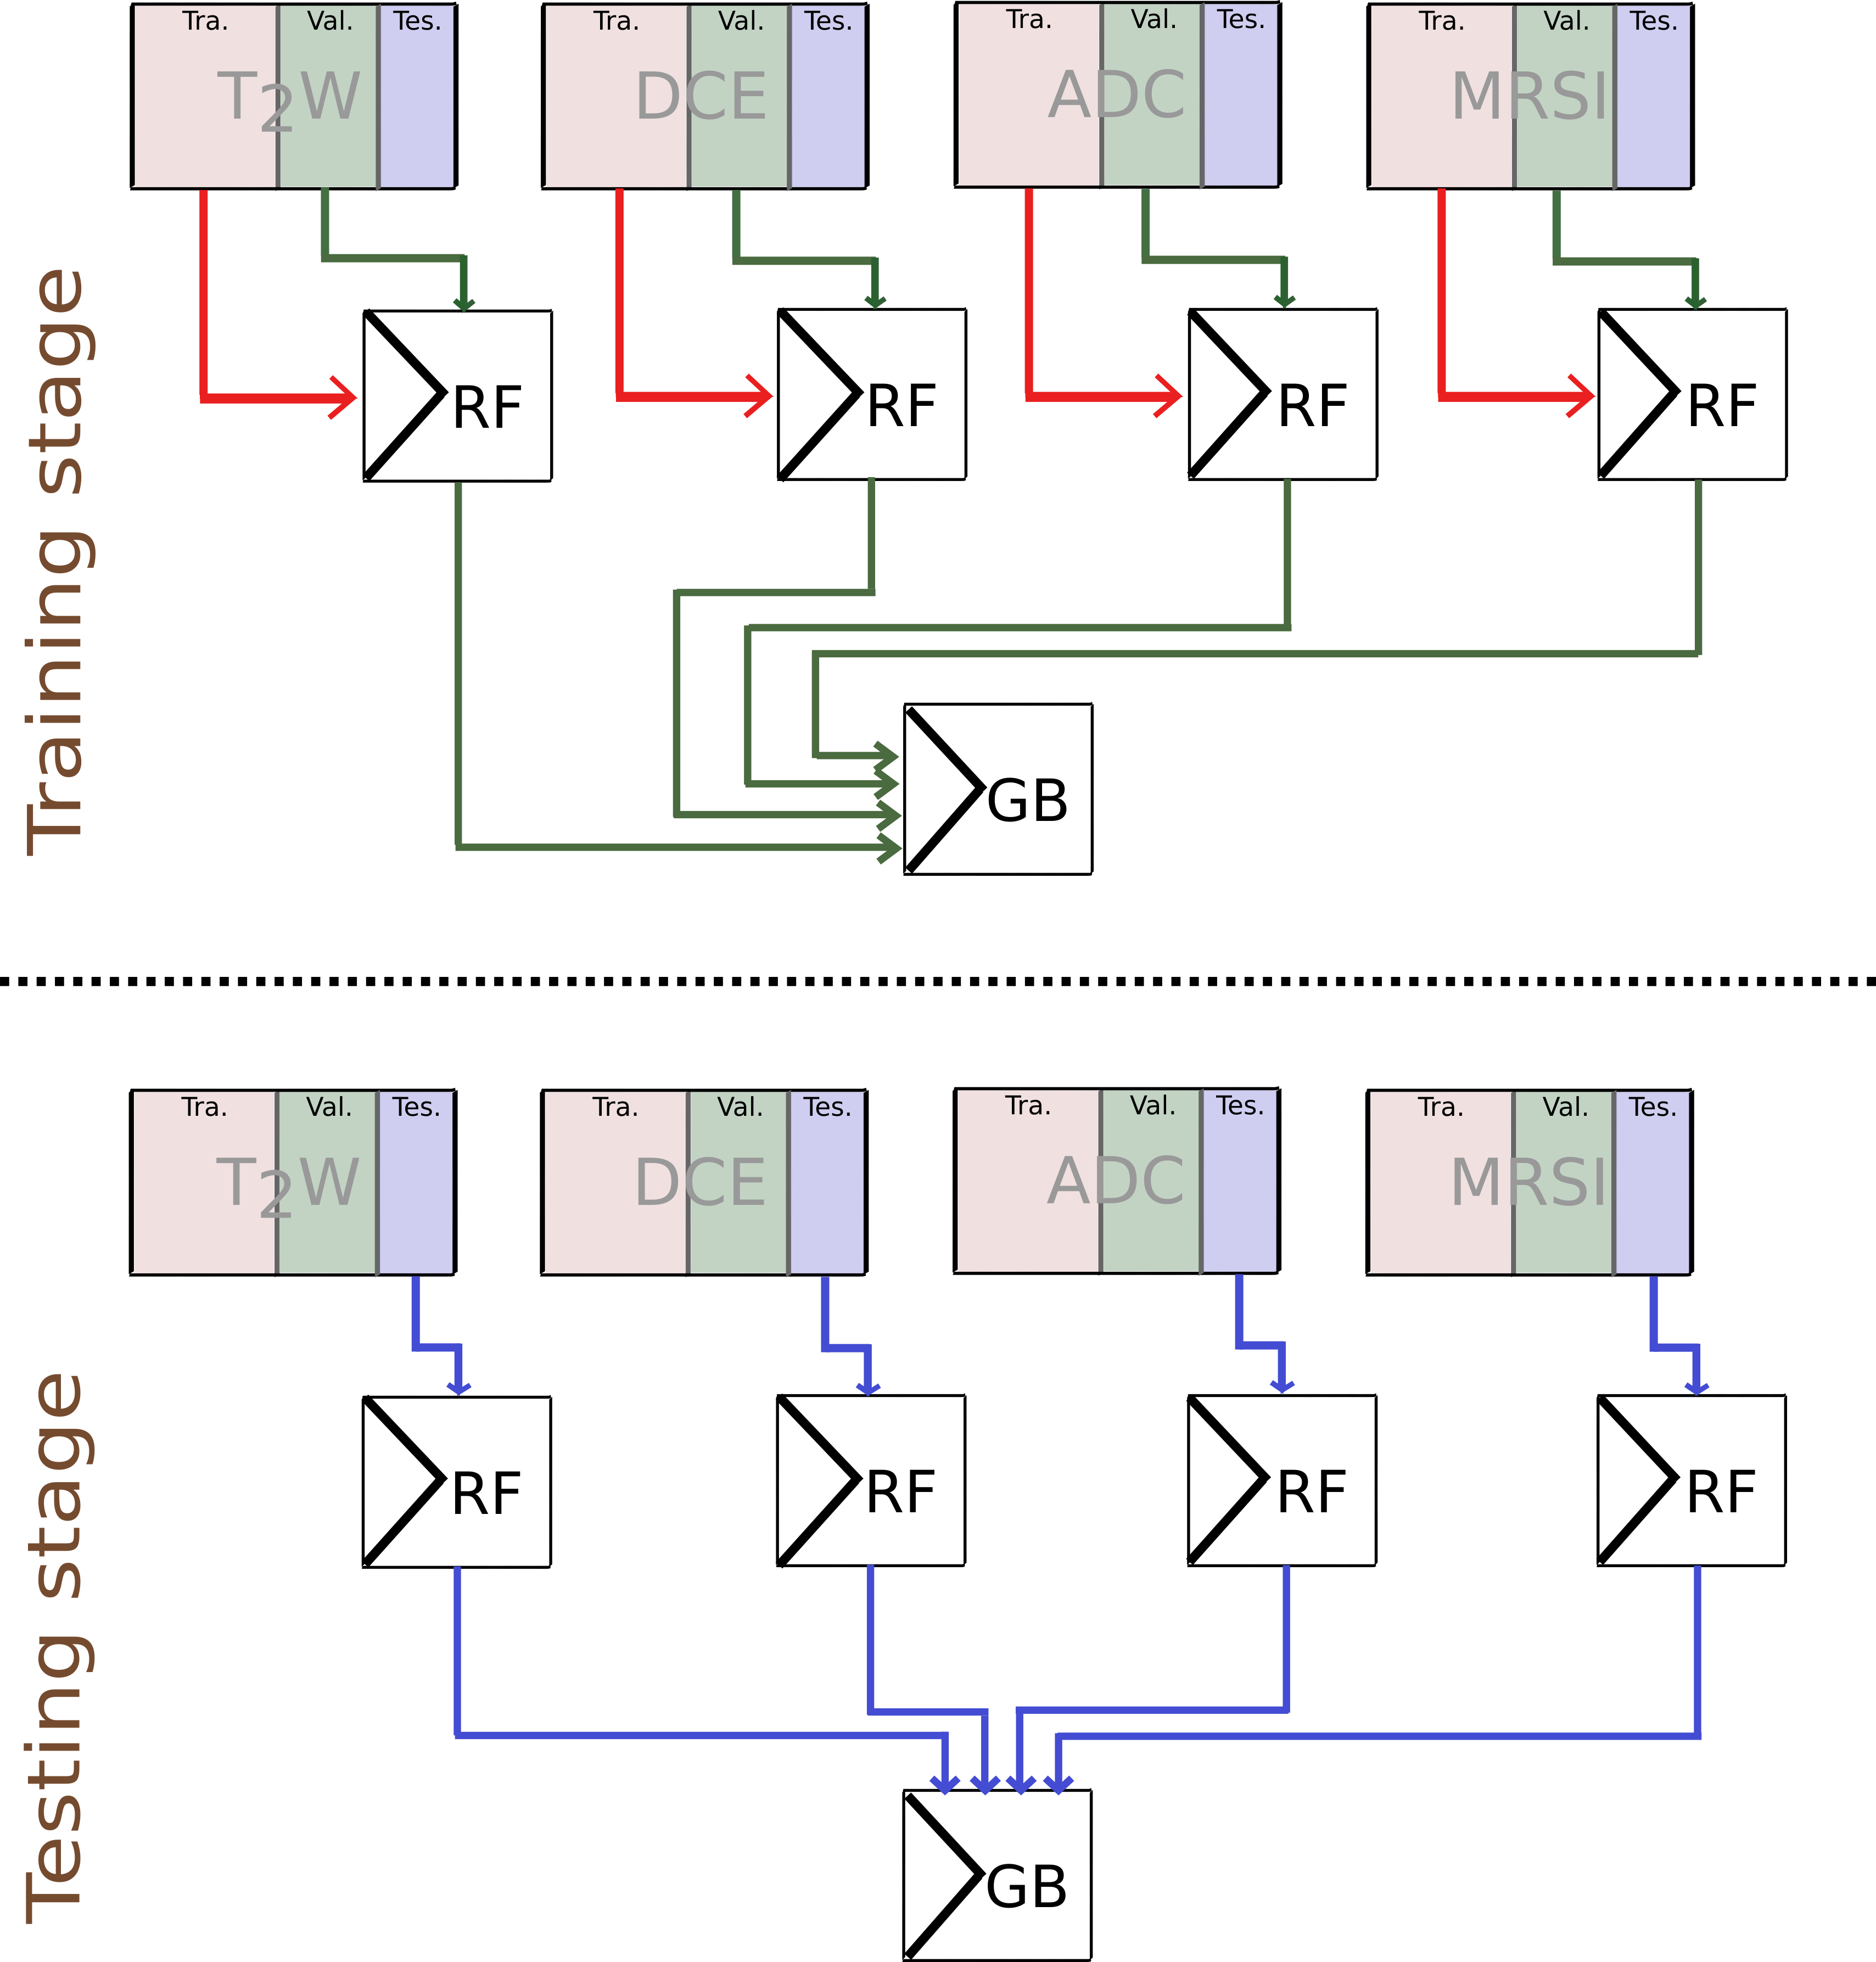
\includegraphics[width=0.5\linewidth]{content/figures/stacking_gb.png}
  \caption[The principle of stacking.]{The principle of stacking. First, training samples (red) are used to train each individual \ac{rf}. Subsequently, a validation set (green) is provided to each \ac{rf} which outputs a set of probabilities used for the classification of the meta-classifier. Finally, a test set is used to asses the classification performance to whole stack.}
  \label{fig:stacking}
\end{figure}

Additionally, we use stacking to create ensemble of base learners using a meta-classifier~\cite{wolpert1992stacked}.
\Acl{fig}~\ref{fig:stacking} illustrate the principle of stacking.
Stacking consists in a two-stage learning:
(i) First, a set of training samples is used to train each individual base learner and
(ii) subsequently, a set of validation samples is provided to each \ac{rf} which individually output a corresponding set of probability used to train a meta-classifier.
Finally, the stack of classifiers is assessed by providing a test set which is going through the base learners and the meta-classifier.

In the later experiments, \ac{adb} and \ac{gb} are chosen as meta-classifiers to aggregate the base learners in the stacking strategies.
\ac{adb} has been presented in \acs{sec}\,\ref{subsec:chp3:img-clas:CADX-clas} and thus only \ac{gb} will be succinctly in the remaining of this section.
\ac{gb} is an ensemble classifier~\cite{friedman2001greedy} which similarly to \ac{adb} is formulated as in \acs{eq}\,\eqref{eq:gbadd}.

\begin{equation}
  F(x) = \sum_{m=1}^{M} \gamma_{m} h_m(x) \ ,
  \label{eq:gbadd}
\end{equation}

\noindent where $h_m(x)$ is a weak learner with its associated weight $\gamma_m$.
As with \ac{adb}, $h_m(x)$ is chosen to minimize a loss function using the additive model $F_{m-1}$.
The difference between \ac{adb} and \ac{gb} lie in the fact the this minimization is tackle as a numerical optimization problem using the steepest descent.


\section{Experiments and results}\label{sec:chp6:exp-res}

In this section, different experiments are proposed to design and investigate our \ac{mpmri} \ac{cad} for the detection of \ac{cap}.
First, the classification performance of each independent modality is investigated in \acs{sec}\,\ref{subec:chp6:exp-res:Ex1}.
For each modality, the ``quantification'' approaches maximizing the classification performance are selected.
Additionally, we focus on to directly combined \ac{mpmri} modalities, which we referred to as ``coarse'' combination as presented in \acs*{sec}\,\ref{subsec:chp6:exp-res:Ex2}.
Subsequently, \acs{sec}\,\ref{subsec:chp6:exp-res:Ex3} presents the benefit of balancing the dataset on the learning stage and strategies for feature selection and extraction, for each feature modality as well as an aggregation of them.
Consequently, different combination classifier rules are studied using the previous fine-tuned feature space in \acs{sec}\,\ref{subsec:chp6:exp-res:Ex4}.
Finally, we conclude in \acs{sec}\,\ref{subsec:chp6:exp-res:Ex5} by investigating the benefit of fusing the \ac{mrsi} information with the other modality.

All these experiments are conducted on a subset of the public \ac{mpmri} prostate presented in \acs{sec}\,\ref{sec:data3t}.
We used the \SI{3}{\tesla} dataset which is composed of a total of 19 patients of which 17 patients had biopsy proven \ac{cap} and 2 patients are ``healthy'' with negative biopsies. 
In this study, our subset consists of 17 patients with \ac{cap}.

\begin{landscape}
\begin{figure}
  \hspace*{\fill}
  \subfigure[Performance of the quantitative methods on \acs*{dce}-\acs*{mri}.]{\label{fig:inddcemodel}\includegraphics[height=.4\textheight]{5_normalization/figures/DCE-normalization/normalized_methods_0.pdf}}
  \hfill
  \subfigure[Performance of enhanced \acs*{dce}-\acs*{mri} signal.]{\label{fig:inddcesignal}\includegraphics[height=.4\textheight]{5_normalization/figures/DCE-normalization/full_signal_0.pdf}}
  \hspace*{\fill} \\
  \hspace*{\fill}
  \subfigure[Performance of image-based features for \acs*{t2w}-\acs*{mri} and \acs*{adc} map.]{\label{fig:indadct2w}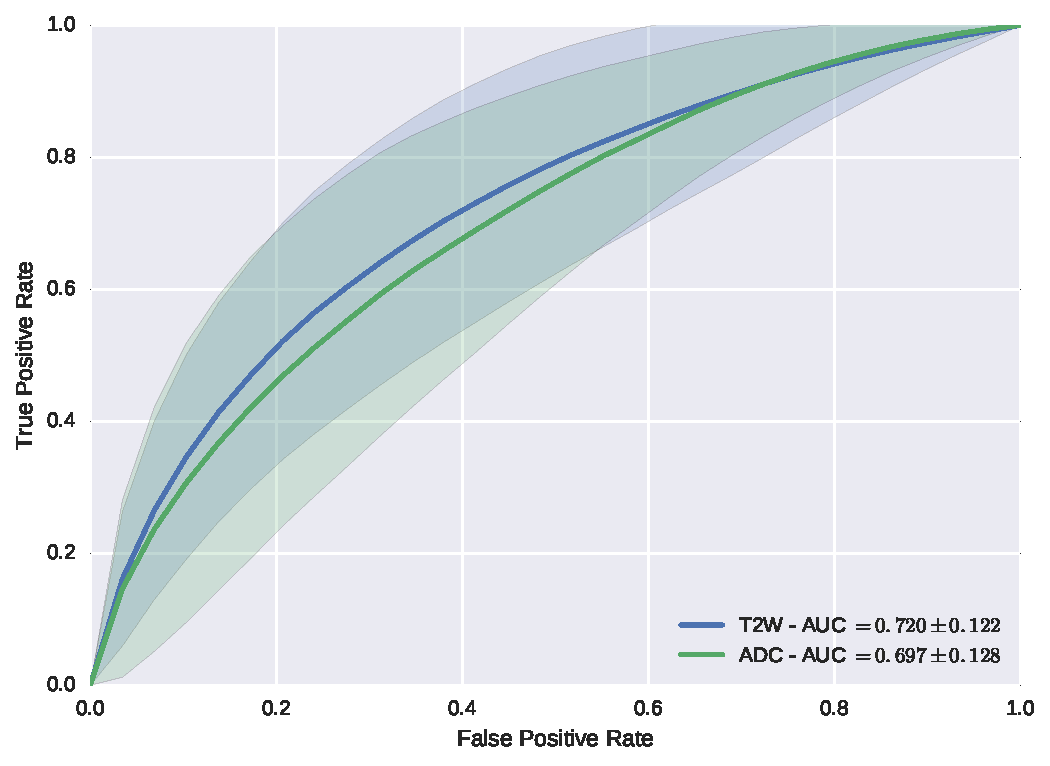
\includegraphics[height=.4\textheight]{content/figures/exp-1/t2w_adc.pdf}}
  \hfill
  \subfigure[Performance of different approaches for the \acs*{mrsi} modality.]{\label{fig:indmrsi}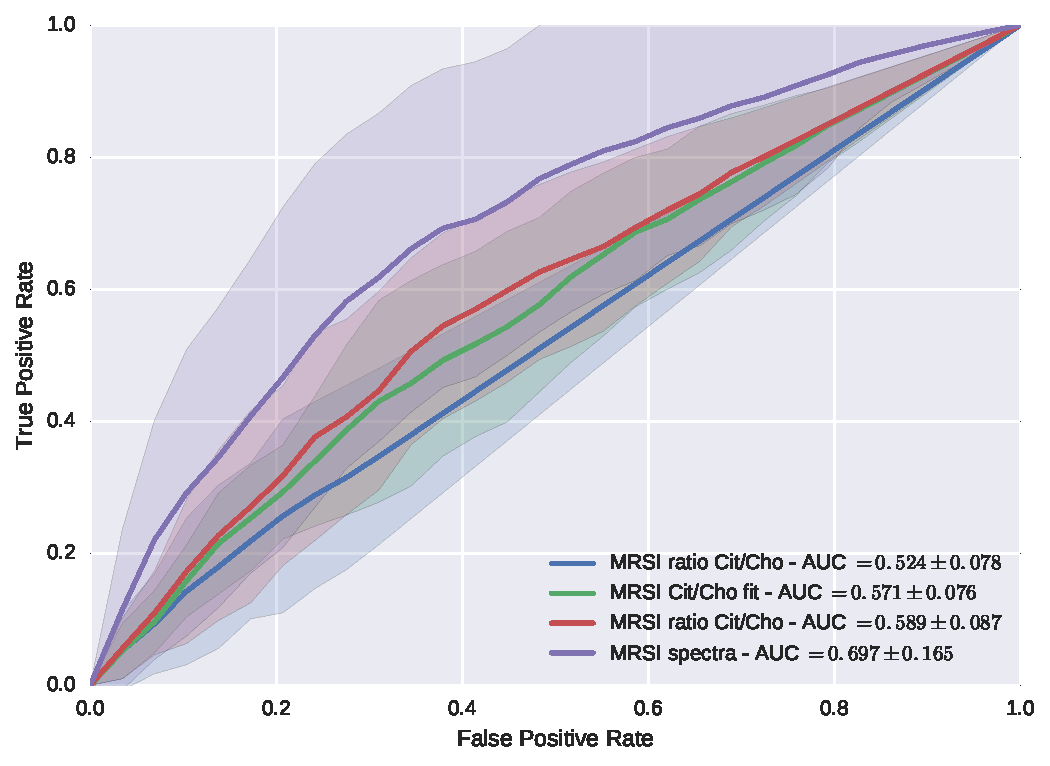
\includegraphics[height=.4\textheight]{content/figures/exp-1/mrsi_all.pdf}}
  \hspace*{\fill}
  \caption[Analysis of the classification performance for each individual \acs*{mri} modality.]{Analysis of the classification performance for each individual \acs*{mri} modality. Different models have been tested for \acs*{dce}-\acs*{mri} and \acs*{mrsi} modalities.}
  \label{fig:res-Ex1}
\end{figure}
\end{landscape}

\subsection{Assessment of classification performance of individual modality}\label{subec:chp6:exp-res:Ex1}

In this experiment, we attend to assess the classification performance of each individual \ac{mri} modality.

\paragraph{\ac{t2w}-\ac{mri} and \ac{adc} map features} All features presented in \acs{tab}~\ref{tab:featureadct2w} are extracted for both \ac{t2w}-\ac{mri} and \ac{adc} map.
These features are combined per modality and for each of them, a \ac{rf} classifier is trained.

\paragraph{\ac{dce}-\ac{mri} features} This experiment has been presented in \acs{sec}\,\ref{subsec:chp5:DCE-norm:exp-res}.
We aim at finding the most discriminative ``quantification'' method for \ac{dce}-\ac{mri} modality, by assessing the classification performance of the different models.
Therefore, the pharmacokinetic parameters from the Brix, Hoffmann, Tofts, and \ac{pun} models, the semi-quantitative parameters, and the enhanced \ac{dce}-\ac{mri} signal are extracted.
For each set of feature, a \ac{rf} classifier is trained.

\paragraph{\ac{mrsi} features} Similarly to \ac{dce}-\ac{mri}, 4 \ac{rf} classifiers are trained on different features:
(i) the cropped \ac{mrsi} signal,
(ii) the relative concentration of the citrate over the relative concentration of the choline, both computed through fitting as presented in the previous section,
(iii) the ratio of the two previous features, and finally
(iv) the ratio of the relative concentration of the citrate over the relative concentration of the choline, using fix integration bounds.

\paragraph{Results}
Each trained \ac{rf} is evaluated using a \ac{lopo}.
A \ac{roc} analysis is carried out and the \ac{auc} score is computed to report and compare the classification performance of each classifier.
The results are depicted in \acs{fig}\,\ref{fig:res-Ex1}.
As presented is the previous chapter, classification of \ac{dce}-\ac{mri} data using the normalized enhanced \ac{dce}-\ac{mri} signal is the strategy leading the highest \ac{auc} --- i.e., $0.666 \pm 0.154$ ---, outperforming any quantification method.
Similarly to these findings, classification of the cropped \ac{mrsi} signal outperforms other quantification-based methods, with an \ac{auc} of $0.697 \pm 0.165$.
Classification of the extracted features based on \ac{adc} offer a close performance with an identical mean \ac{auc} and a smaller standard deviation of $0.128$.
Finally, the features extracted from \ac{t2w}-\ac{mri} are shown to be the most discriminative with an \ac{auc} reaching $0.720 \pm 0.122$.
As a conclusion, the most efficient features in terms of classification performance for each modality are selected for the remainder of the experiment section.

\subsection{Coarse combination of \acs*{mpmri} modalities} \label{subsec:chp6:exp-res:Ex2}

\begin{figure}
  \centering
  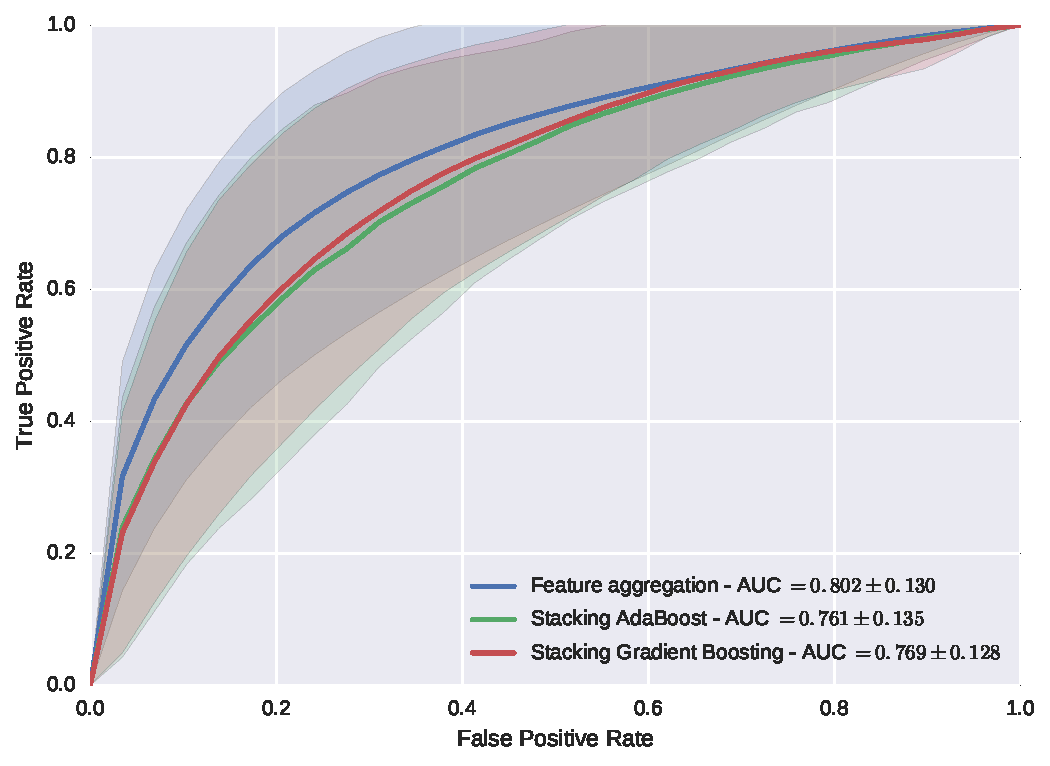
\includegraphics[width=0.7\linewidth]{content/figures/exp-2/comb_all.pdf}
  \caption[Comparison of different combination approaches.]{Comparison of different combination approaches: (i) aggregation of the different features in conjunction with a \acs*{rf} classifier, (ii) a stacking approach using 4 \acs*{rf}s and \acs*{adb} as meta-classifier, and (iii) a stacking approach using 4 \acs*{rf}s and \acs*{gb} as meta-classifier.}
  \label{fig:res-Exp2}
\end{figure}

As a first attempt to design a \ac{mpmri} \ac{cad} system, 3 different approaches are used to combine the selected feature from each modality:
(i) feature aggregation,
(ii) stacking using \ac{adb},
(iii) stacking using \ac{gb}.
We refer these combinations as being coarse since no tuning --- i.e., feature balancing/selection/extraction --- aiming at improving the classification performance is involved.
This experiment can be considered as the baseline to obtain a \ac{mpmri} \ac{cad} for the detection of \ac{cap}.

In the first approach, the features from all the different modalities are concatenated together to form a unique matrix.
Additionally, the anatomical features are concatenated within the same matrix.
The second and third approaches are based on the stacking which has been presented in the previous section.
They differ in the choice of the meta-learner since the first stack uses an \ac{adb} classifier while the second stack uses a \ac{gb}.
Each base learner is similar to the \ac{rf} selected in the previous experiment.
The difference lie in the concatenation of the anatomical features with each feature set derived from the \ac{mri} modality presented in the previous experiment.

\paragraph{Results}
The three coarse combinations are tested using a \ac{lopo}.
Furthermore, for the stacking approaches, the training set is split into a smaller training set and a validation set composed of 10 and 6 patients, respectively.
A \ac{roc} analysis is carried out for each combination and the \ac{auc} is computed as reported in \acs{fig}\,\ref{fig:res-Exp2}.

A single learner using aggregated features outperforms the stacking-based classifier with an \ac{auc} of $0.802 \pm 0.130$.
Furthermore, \ac{gb} chosen as a meta-classifier leads to better classification performance than \ac{adb}, with an improved \ac{auc} from $0.761 \pm 0.135$ to $0.769 \pm 0.128$.

\subsection{Benefits of data balancing and feature selection/extraction}\label{subsec:chp6:exp-res:Ex3}

In this section, we focus on optimizing the different feature set used in the previous classification.
Therefore, our contribution is twofold: (i) we compare the different balancing methods to distinguish which method is the best suited and (ii) we use feature selection/extraction methods to identify which feature are the most discriminative among each set.

\begin{figure}
  \centering
  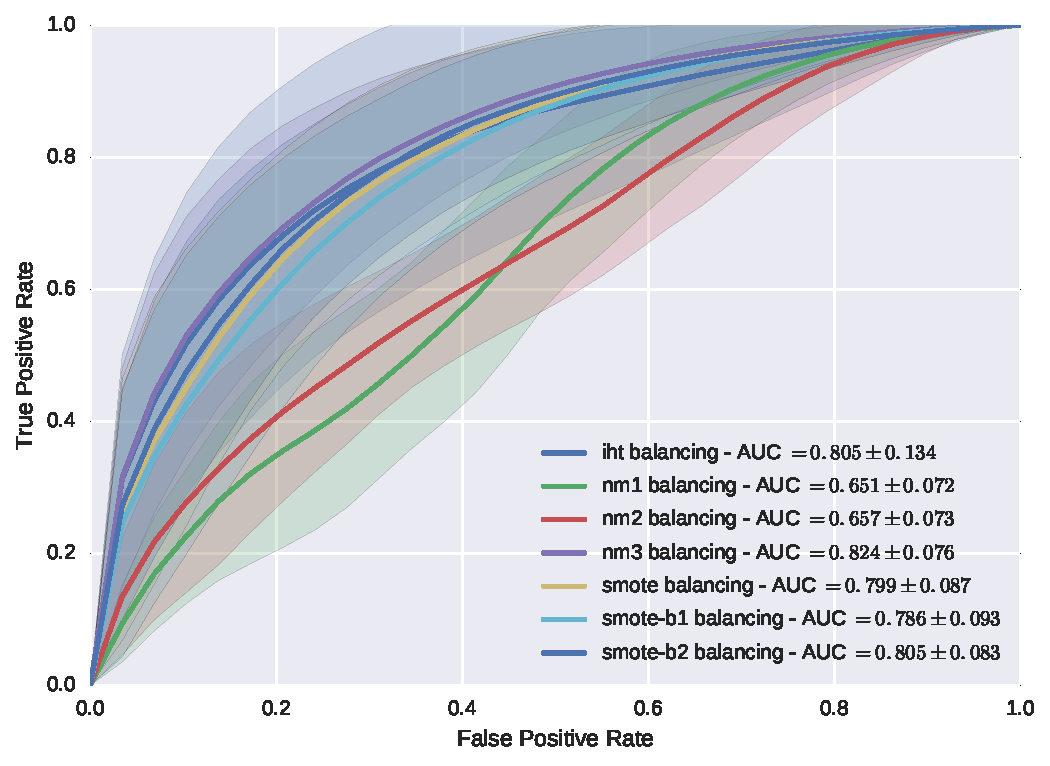
\includegraphics[width=0.7\linewidth]{content/figures/exp-3/all.pdf}
  \caption{Analysis of the benefit of balancing the training dataset before the learning process while concatenating all features.}
  \label{fig:allbalance}
\end{figure}

\paragraph{Comparison of balancing strategies}
For this experiment, a \ac{rf} classifier is trained for each feature set selected from the first experiment.
As in the previous experiment, a \ac{lopo} is used as validation model.
During the learning phase, the training sets are balanced using the methods presented in \acs{sec}\,\ref{subsec:chp6:method:fea-bal}.
The possible improvements offered by the balancing methods is analyzed through a \ac{roc} analysis and computing the \ac{auc}.
The results are depicted in \acs{fig}\,\ref{fig:res-Ex3-bal} and give rise to two observations:
(i) there is at least one balancing method which improves the classification performance and
(ii) \ac{iht} and \ac{smote} are the methods performing the best on individual modality features.
On the one hand, \ac{iht} outperforms the other methods while balancing the feature sets based on the \ac{dce}-\ac{mri} and \ac{adc} map.
The \ac{auc} increases of $0.019$ and $0.018$ for the feature sets of the \ac{dce}-\ac{mri} and \ac{adc} map, respectively.
On the other hand, \ac{smote} increases the \ac{auc} of $0.042$ for \ac{t2w}-\ac{mri}.
However, there is no significant improvement for the \ac{mrsi} since only the standard deviation of the \ac{auc} decreases of $0.019$.
Once all features are concatenated together, \ac{nm3} is the method providing the best enhancement of the classification performance with an \ac{auc} of $0.824 \pm 0.076$, as depicted in \acs{fig}\,\ref{fig:allbalance}.
In conclusion, the methods leading to the best performance are applied prior to feature selection/extraction for the remainder of the experiment.

\paragraph{Feature selection and extraction}

Noisy or non-discriminative features included in the learning process might degrade the overall performance of a classifier.
Thus, the feature selection and extraction methods presented in \acs{sec}\,\ref{subsec:chp6:method:fea-bal} are used to obtain a fine-tuned feature space.
The selection approaches --- i.e., \ac{anova} F-value and Gini importance --- are applied on the image-based features extracted from \ac{t2w}-\ac{mri} and \ac{adc} map modalities.
For both methods, a threshold defines the percentage of features to select.
Additionally, several thresholds are defined to find the number of features maximizing the classification performance.

Features computed from \ac{mrsi} and \ac{dce}-\ac{mri} modalities are related to signal and feature extraction seems more appropriate rather than feature selection.
Therefore, the 3 feature extraction methods --- i.e., \ac{pca}, sparse-\ac{pca}, and \ac{ica} --- are applied by varying the number of components or the sparsity level, which allows to find the level which maximizes the classification performance.
Finally, the feature selection methods have been applied on the concatenation of all the features.

\begin{landscape}
\begin{figure}
  \hspace*{\fill}
  \subfigure[\ac{t2w}-\ac{mri}]{\label{fig:ex3:T2W}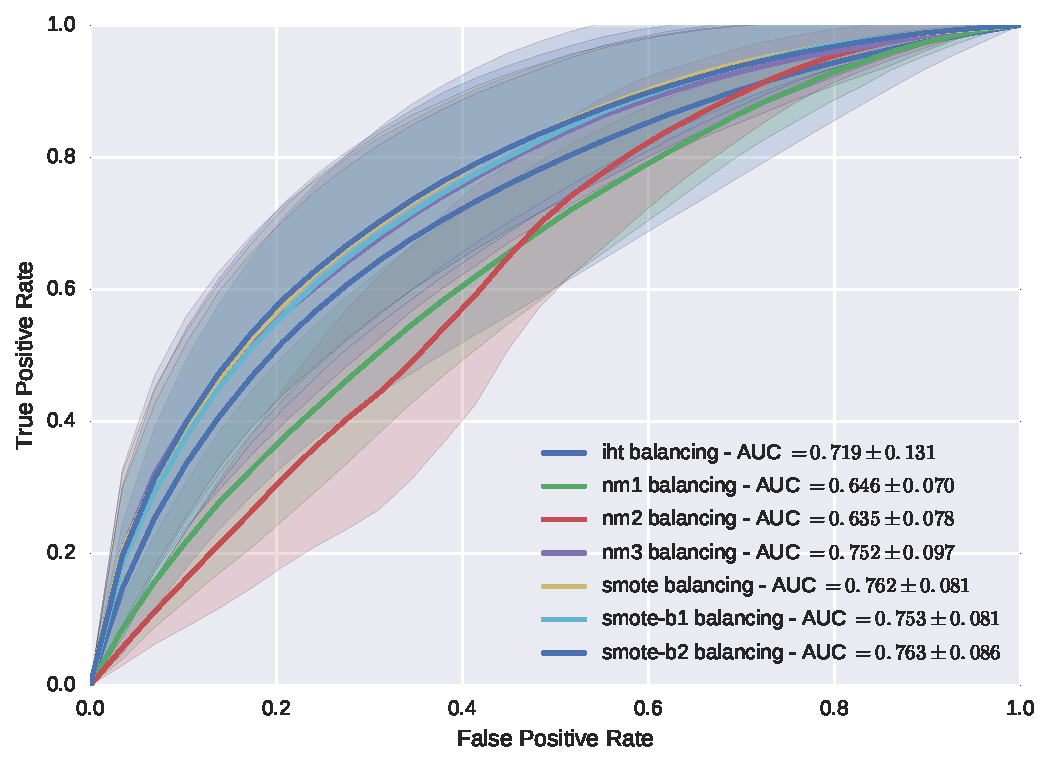
\includegraphics[height=.4\textheight]{content/figures/exp-3/t2w.pdf}}
  \hfill
  \subfigure[\ac{adc}-\ac{mri}]{\label{fig:ex3:ADC}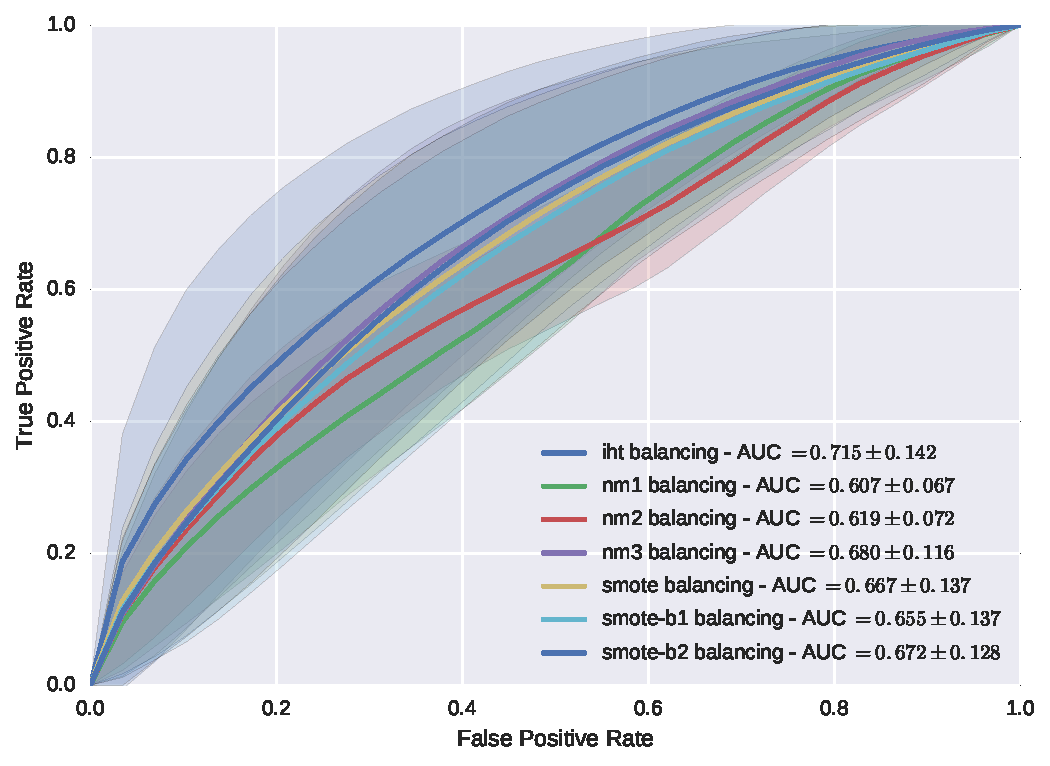
\includegraphics[height=.4\textheight]{content/figures/exp-3/adc.pdf}}
  \hspace*{\fill} \\
  \hspace*{\fill}
  \subfigure[\ac{dce}-\ac{mri}]{\label{fig:ex3-DCE}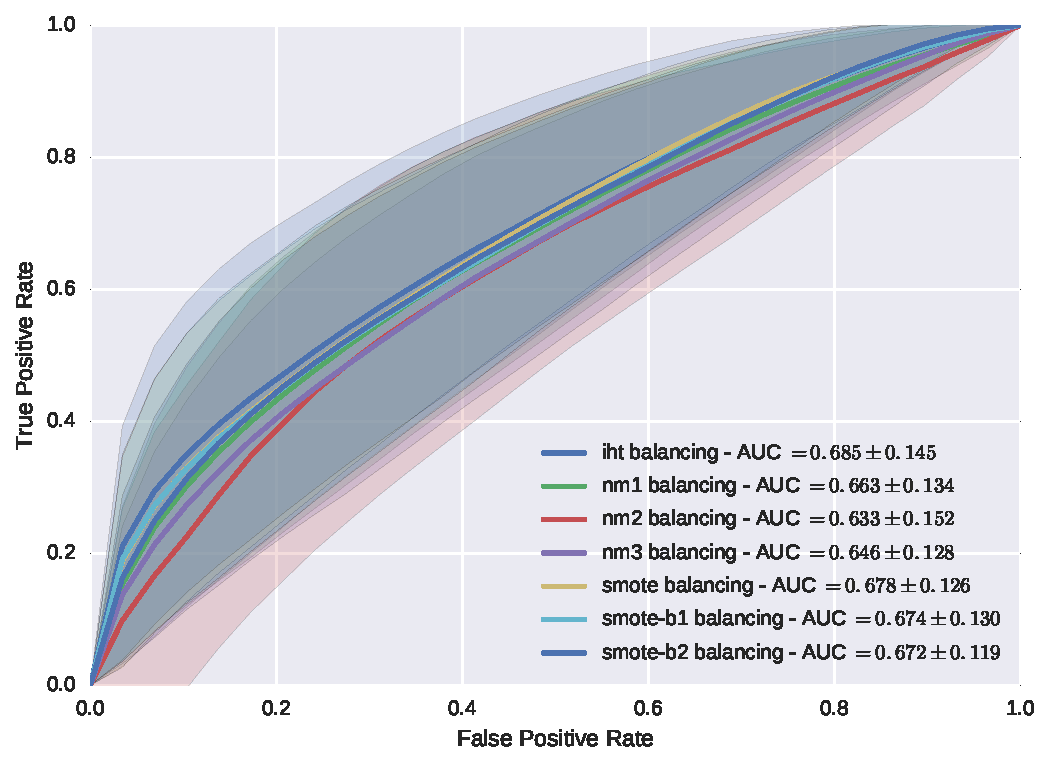
\includegraphics[height=.4\textheight]{content/figures/exp-3/dce.pdf}}
  \hfill
  \subfigure[\ac{mrsi}-\ac{mri}]{\label{fig:ex3-MRSI}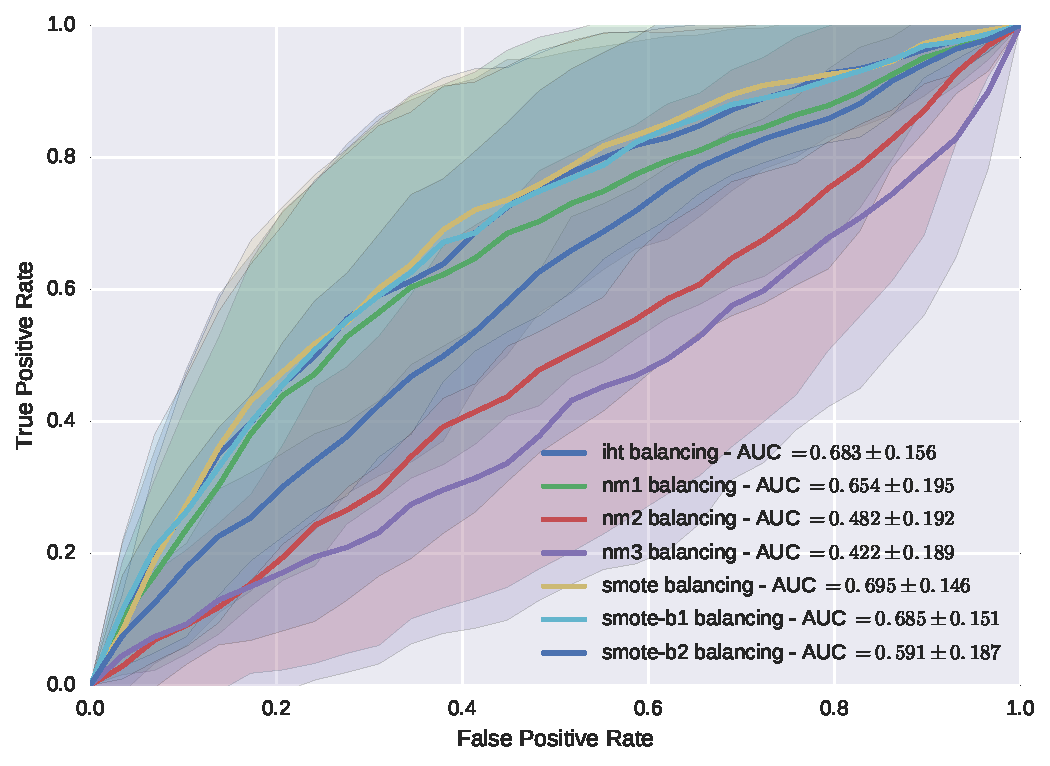
\includegraphics[height=.4\textheight]{content/figures/exp-3/mrsi.pdf}}
  \hspace*{\fill}
  \caption{Analysis of the benefit of balancing the training dataset before learning process for each modality.}
  \label{fig:res-Ex3-bal}
\end{figure}

\begin{table}
  \caption{Results in terms of \acs*{auc} of the feature selection based on \acs*{anova} F-value for \acs*{t2w}-\acs*{mri}.}
  \centering
  \scriptsize
  \begin{tabularx}{\linewidth}{@{}l >{\centering\arraybackslash}X >{\centering\arraybackslash}X >{\centering\arraybackslash}X >{\centering\arraybackslash}X >{\centering\arraybackslash}X >{\centering\arraybackslash}X >{\centering\arraybackslash}X @{}}
    \toprule
    \multirow{2}{*}{\textbf{Methods}} & \multicolumn{7}{c}{\textbf{Percentiles}} \\
    \cmidrule{2-8}
    & 15 & 17.5 & 20 & 22.5 & 25 & 27.5 & 30 \\
    \midrule
    \acs*{anova} F-score & $0.755 \pm 0.049$ & $0.770 \pm 0.058$ & $0.777 \pm 0.064$ & $0.782 \pm 0.066$ & $\mathbf{0.784 \pm 0.067}$ & $0.783 \pm 0.072$ & $0.782 \pm 0.070$ \\
    \bottomrule
  \end{tabularx}
  \label{tab:ginit2w}
\end{table}

\begin{table}
  \caption{Results in terms of \acs*{auc} of the feature selection based on Gini importance for \acs*{t2w}-\acs*{mri}.}
  \centering
  \scriptsize
  \begin{tabularx}{\linewidth}{@{}l >{\centering\arraybackslash}X >{\centering\arraybackslash}X >{\centering\arraybackslash}X >{\centering\arraybackslash}X >{\centering\arraybackslash}X >{\centering\arraybackslash}X >{\centering\arraybackslash}X @{}}
    \toprule
    \multirow{2}{*}{\textbf{Methods}} & \multicolumn{7}{c}{\textbf{Percentiles}} \\
    \cmidrule{2-8}
    & 1 & 2 & 5 & 10 & 15 & 20 & 30 \\
    \midrule
    Gini importance & $0.726 \pm 0.064$ & $0.731 \pm 0.055$ & $0.751 \pm 0.065$ & $0.758 \pm 0.076$ & $0.752 \pm 0.087$ & $0.761 \pm 0.077$ & $\mathbf{0.764 \pm 0.079}$ \\
    \bottomrule
  \end{tabularx}
  \label{tab:anovat2w}
\end{table}

\begin{table}
  \caption{Results in terms of \acs*{auc} of the feature selection based on \acs*{anova} F-value for \acs*{adc}.}
  \centering
  \scriptsize
  \begin{tabularx}{\linewidth}{@{}l >{\centering\arraybackslash}X >{\centering\arraybackslash}X >{\centering\arraybackslash}X >{\centering\arraybackslash}X >{\centering\arraybackslash}X >{\centering\arraybackslash}X >{\centering\arraybackslash}X @{}}
    \toprule
    \multirow{2}{*}{\textbf{Methods}} & \multicolumn{7}{c}{\textbf{Percentiles}} \\
    \cmidrule{2-8}
    & 10 & 12.5 & 15 & 17.5 & 20 & 22.5 & 25 \\
    \midrule
    \acs*{anova} F-score & $0.684 \pm 0.123$ & $0.713 \pm 0.125$ & $0.712 \pm 0.134$ & $0.710 \pm 0.144$ & $\mathbf{0.714 \pm 0.142}$ & $0.708 \pm 0.150$ & $0.708 \pm 0.150$ \\
    \bottomrule
  \end{tabularx}
  \label{tab:giniadc}
\end{table}

\begin{table}
  \caption{Results in terms of \acs*{auc} of the feature selection based on Gini importance for \acs*{adc} map.}
  \centering
  \scriptsize
  \begin{tabularx}{\linewidth}{@{}l >{\centering\arraybackslash}X >{\centering\arraybackslash}X >{\centering\arraybackslash}X >{\centering\arraybackslash}X >{\centering\arraybackslash}X >{\centering\arraybackslash}X >{\centering\arraybackslash}X @{}}
    \toprule
    \multirow{2}{*}{\textbf{Methods}} & \multicolumn{7}{c}{\textbf{Percentiles}} \\
    \cmidrule{2-8}
    & 1 & 2 & 5 & 10 & 15 & 20 & 30 \\
    \midrule
    Gini importance & $0.672 \pm 0.132$ & $0.690 \pm 0.138$ & $\mathbf{0.743 \pm 0.139}$ & $0.730 \pm 0.136$ & $0.730 \pm 0.142$ & $0.724 \pm 0.141$ & $0.722 \pm 0.142$ \\
    \bottomrule
  \end{tabularx}
  \label{tab:anovaadc}
\end{table}

\begin{table}
  \caption{Results in terms of \acs*{auc} of the feature extraction methods for \acs*{dce}-\ac{mri}.}
  \centering
  \scriptsize
  \begin{tabularx}{\linewidth}{@{}l >{\centering\arraybackslash}X >{\centering\arraybackslash}X >{\centering\arraybackslash}X >{\centering\arraybackslash}X >{\centering\arraybackslash}X >{\centering\arraybackslash}X >{\centering\arraybackslash}X @{}}
    \toprule
    \multirow{2}{*}{\textbf{Methods}} & \multicolumn{7}{c}{\textbf{Number of components or sparsity level}} \\
    \cmidrule{2-8}
    & 2 & 4 & 8 & 16 & 24 & 32 & 36 \\
    \midrule
    \acs*{pca} & $0.656 \pm 0.133$ & $0.634 \pm 0.121$ & $0.668 \pm 0.149$ & $0.680 \pm 0.145$ & $0.682 \pm 0.146$ & $0.679 \pm 0.151$ & $0.683 \pm 0.149$ \\
    Sparse-\acs*{pca} & $0.578 \pm 0.117$ & $0.546 \pm 0.121$ & $0.554 \pm 0.097$ & --- & --- & --- & --- \\
    \acs*{ica} & $0.657 \pm 0.132$ & $0.629 \pm 0.117$ & $0.671 \pm 0.157$ & $0.686 \pm 0.158$ & $\mathbf{0.691 \pm 0.158}$ & $0.681 \pm 0.161$ & $0.679 \pm 0.166$ \\
    \bottomrule
  \end{tabularx}
  \label{tab:dcefeatext}
\end{table}


\begin{table}
  \caption{Results in terms of \acs*{auc} of the feature extraction methods for \acs*{mrsi}.}
  \centering
  \scriptsize
  \begin{tabularx}{\linewidth}{@{}l >{\centering\arraybackslash}X >{\centering\arraybackslash}X >{\centering\arraybackslash}X >{\centering\arraybackslash}X >{\centering\arraybackslash}X >{\centering\arraybackslash}X >{\centering\arraybackslash}X @{}}
    \toprule
    \multirow{2}{*}{\textbf{Methods}} & \multicolumn{7}{c}{\textbf{Number of components or sparsity level}} \\
    \cmidrule{2-8}
    & 2 & 4 & 8 & 16 & 24 & 32 & 36 \\
    \midrule
    \acs*{pca} & $0.566 \pm 0.120$ & $0.575 \pm 0.141$ & $0.648 \pm 0.162$ & $0.662 \pm 0.177$ & $0.659 \pm 0.184$ & $0.671 \pm 0.179$ & $0.672 \pm 0.182$ \\
    Sparse-\acs*{pca} & $0.502 \pm 0.050$ & $0.571 \pm 0.158$ & $0.585 \pm 0.111$ & --- & --- & --- & --- \\
    \acs*{ica} & $0.567 \pm 0.119$ & $0.578 \pm 0.140$ & $0.654 \pm 0.145$ & $0.656 \pm 0.167$ & $0.650 \pm 0.187$ & $0.663 \pm 0.174$ & $\mathbf{0.677 \pm 0.171}$ \\
    \bottomrule
  \end{tabularx}
  \label{tab:mrsifeatext}
\end{table}

\begin{table}
  \caption{Results in terms of \acs*{auc} of the feature selection based on \acs*{anova} F-value for the aggregation of feature from all \acs*{mpmri} features.}
  \centering
  \scriptsize
  \begin{tabularx}{\linewidth}{@{}l >{\centering\arraybackslash}X >{\centering\arraybackslash}X >{\centering\arraybackslash}X >{\centering\arraybackslash}X >{\centering\arraybackslash}X >{\centering\arraybackslash}X >{\centering\arraybackslash}X @{}}
    \toprule
    \multirow{2}{*}{\textbf{Methods}} & \multicolumn{7}{c}{\textbf{Percentiles}} \\
    \cmidrule{2-8}
    & 10 & 12.5 & 15 & 17.5 & 20 & 22.5 & 25 \\
    \midrule
    \acs*{anova} F-score & $0.764 \pm 0.095$ & $0.765 \pm 0.079$ & $0.800 \pm 0.083$ & $0.817 \pm 0.089$ & $\mathbf{0.828 \pm 0.084}$ & $0.822 \pm 0.0.084$ & $0.815 \pm 0.086$ \\
    \bottomrule
  \end{tabularx}
  \label{tab:anovacomb}
\end{table}

\begin{table}
  \caption{Results in terms of \acs*{auc} of the feature selection based on Gini importance for the aggregation of feature from all \acs*{mpmri} features.}
  \centering
  \scriptsize
  \begin{tabularx}{\linewidth}{@{}l >{\centering\arraybackslash}X >{\centering\arraybackslash}X >{\centering\arraybackslash}X >{\centering\arraybackslash}X >{\centering\arraybackslash}X >{\centering\arraybackslash}X >{\centering\arraybackslash}X @{}}
    \toprule
    \multirow{2}{*}{\textbf{Methods}} & \multicolumn{7}{c}{\textbf{Percentiles}} \\
    \cmidrule{2-8}
    & 10 & 12.5 & 15 & 17.5 & 20 & 22.5 & 25 \\
    \midrule
    Gini importance & $0.834 \pm 0.085$ & $0.834 \pm 0.088$ & $0.834 \pm 0.084$ & $\mathbf{0.836 \pm 0.083}$ & $0.834 \pm 0.079$ & $0.828 \pm 0.086$ & $0.830 \pm 0.077$ \\
    \bottomrule
  \end{tabularx}
  \label{tab:ginicomb}
\end{table}

\begin{table}
  \caption{Selected feature and number of occurrence for \acs*{t2w}-\acs*{mri}, \acs*{adc} map, and one all the features are concatenated.}
  \centering
  \scriptsize
  \begin{tabular}{llllll}
    \toprule
    \multicolumn{1}{c}{\textbf{\acs*{t2w}-\acs*{mri}}} & \multicolumn{1}{c}{\textbf{\acs*{adc}}} & \multicolumn{1}{c}{\textbf{\acs*{t2w}-\acs*{mri}}} & \multicolumn{1}{c}{\textbf{\acs*{adc}}} & \multicolumn{1}{c}{\textbf{\acs*{dce}-\acs*{mri}}} & \multicolumn{1}{c}{\textbf{\acs*{mrsi}}} \\
    \cmidrule(lr){1-1} \cmidrule(lr){2-2} \cmidrule(lr){3-6}
    8 edges & 1 \acs*{dct} & 113 Gabor filters & 53 Gabor filters & 14 samples  & 78 samples \\
    155 Gabor filters & 32 Gabor filters & 1 phase congruency & 2 phase congruency & & \\ 
    2 Haralick features & 1 phase congruency & 4 edges & & & \\
    1 intensity & & 1 intensity & & & \\
    4 \acs*{lbp} & & & & & \\
    2 phase congruency & & & & & \\
    \cmidrule(lr){1-1} \cmidrule(lr){2-2} \cmidrule(lr){3-6}
    \multicolumn{1}{c}{\textbf{172 features}} & \multicolumn{1}{c}{\textbf{34 features}} & \multicolumn{4}{c}{\textbf{267 features}} \\
    \bottomrule
  \end{tabular}
  \label{tab:selfeatocc}
\end{table}

\end{landscape}

As the previous experiments, the classification is performed using a \ac{rf} with \ac{lopo} model validation.
A \ac{roc} analysis is performed and for each \ac{roc}, the \ac{auc} score is computed.
The results are reported from \acs{tab}~\ref{tab:ginit2w} to \acs{tab}~\ref{tab:anovacomb}, in which the best results are highlighted in \textbf{bold}.

% feature selection
% results
Overall, feature selection or extraction lead to increase the classification performance.
For features extracted from the \ac{t2w}\ac{mri}, \ac{anova}-based selection lead to better performance than Gini importance selection, with a \ac{auc} of $0.784 \pm 0.067$.
The opposite conclusion is drawn for the features extracted from the \ac{adc} map.
The selection using the Gini importance criterion leads to an \ac{auc} of $0.743 \pm 0.139$.
% improvements
Therefore, the feature selection leads to an improve \ac{auc} of $0.022$ and $0.013$ for \ac{t2w}-\ac{mri} and \ac{adc} map, respectively.
% which features are selected
The features which have been selected are reported in the 1\textsuperscript{st} and 2\textsuperscript{nd} columns of \acs{tab}~\ref{tab:selfeatocc}.
To conclude, from the 690 original features, 172 and 43 features are selected from the \ac{t2w}-\ac{mri} and \ac{adc} map, respectively.

% feature extraction
Regarding feature extraction, \ac{ica} outperforms other methods for both \ac{mrsi} and \ac{dce}-\ac{mri} with \ac{auc} scores of $0.677 \pm 0.171$ and $0.691 \pm 0.158$, respectively.
However, only the projection applied to \ac{dce}-\ac{mri} features leads to improved results with a gain of $0.013$ with 24 components selected instead of the original 40 dimensions.

% feature selection for concatenation
% results
Gini importance selection method is also outperforming \ac{anova}-based method while selecting the features from the concatenation of all of them.
The reported \ac{auc} is $0.836 \pm 0.083$ with an increase of $0.034$.
% which features are selected
The features which have been selected are reported from the 3\textsuperscript{rd} to the 6\textsuperscript{th} columns of \acs{tab}~\ref{tab:selfeatocc}.
To conclude, from the 1533 original features, 267 features are selected from the entire set of feature.

\subsection{Fine-tuned combination of \ac{mpmri} modalities}\label{subsec:chp6:exp-res:Ex4}

\begin{figure}
  \centering
  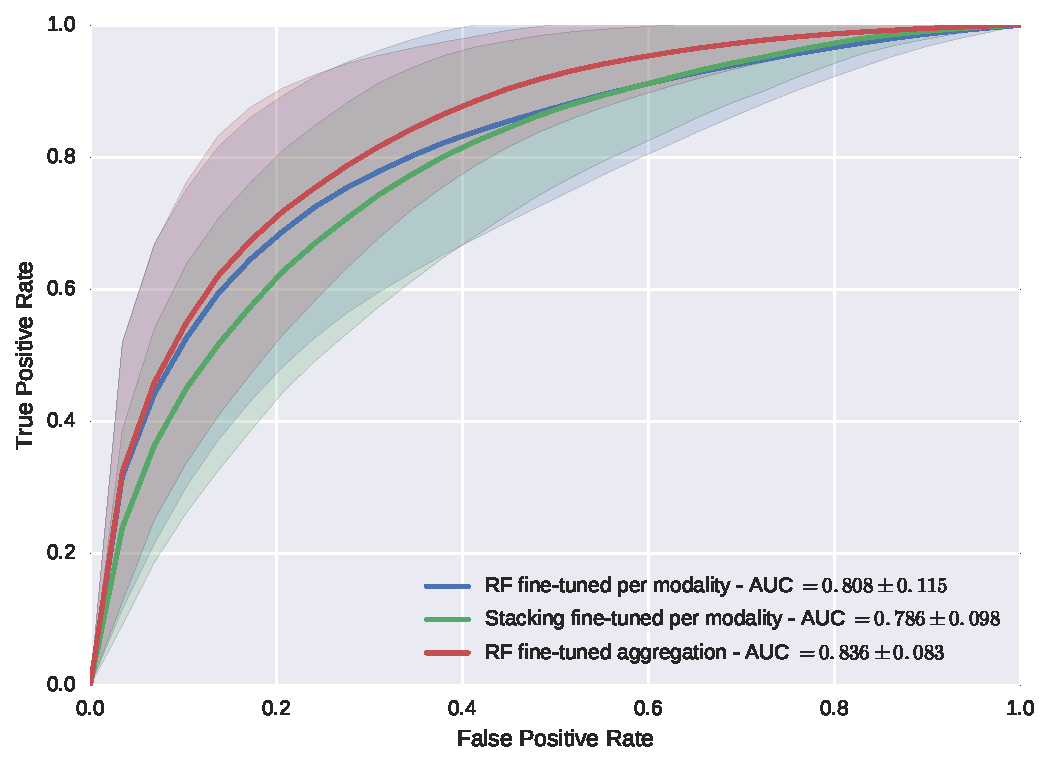
\includegraphics[width=0.7\linewidth]{content/figures/exp-5/combine_all.pdf}
  \caption[Analysis of feature combination approaches after fine tuning.]{Analysis of feature combination approaches after fine tuning through balancing and feature selection/extraction.}
  \label{fig:res-Ex4}
\end{figure}

\begin{figure}
  \centering
  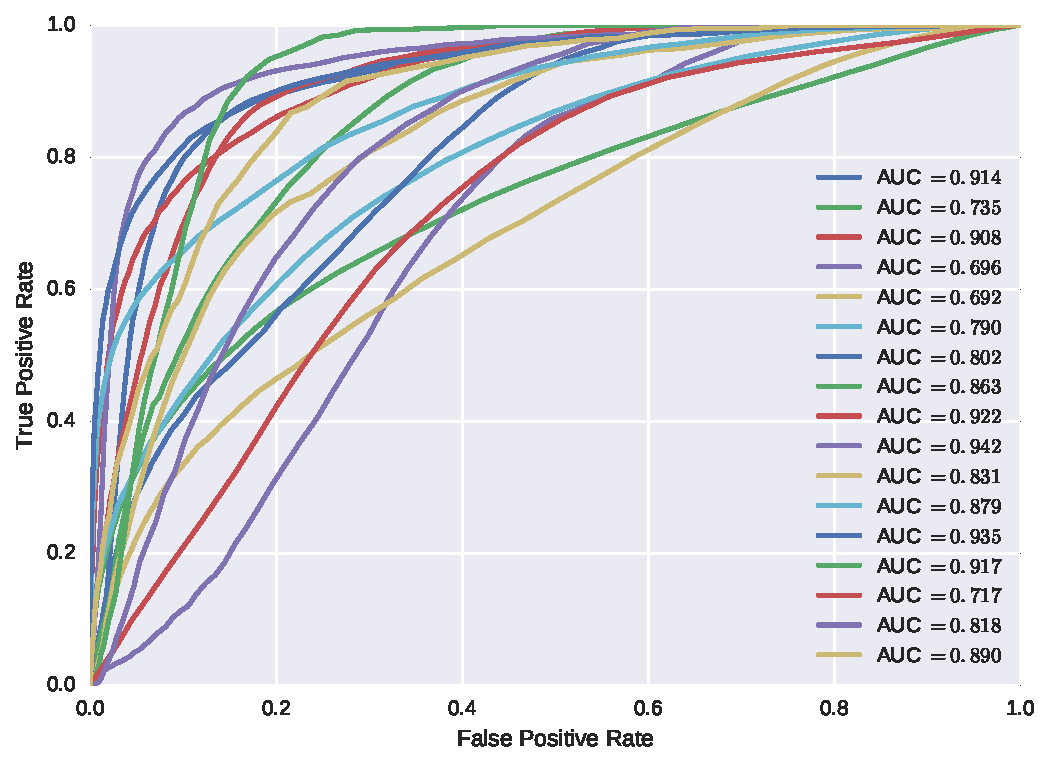
\includegraphics[width=0.7\linewidth]{content/figures/exp-5/plot_all_patients.pdf}
  \caption{Individual patient \acs*{auc} for the best configuration of the \acs*{mpmri} \acs*{cad}.}
  \label{fig:indauc}
\end{figure}

This experiment aims at providing the most efficient \ac{mpmri} \ac{cad} for \ac{cap} using the fine-tuned feature space from the previous experiment.
Three strategies are applied:
(i) the selected features from each modality --- i.e., 331 features --- are concatenated together and used in a \ac{rf} classifier,
(ii) the selected features from each modality --- i.e., 331 features --- are used to train a stacking classifier with a \ac{gb} as meta-classifier, and
(iii) the selected features from the concatenated set of feature --- i.e., 267 features --- are used to train a single \ac{rf} classifier.

\begin{landscape}
\begin{figure}
  \hspace*{\fill}
  \subfigure[\acs*{auc} = 0.922]{\label{fig:pat634}\includegraphics[width=.45\textwidth]{content/figures/examples/patient_634.pdf}}
  \hfill
  \subfigure[\acs*{auc} = 0.942]{\label{fig:pat778}\includegraphics[width=.45\textwidth]{content/figures/examples/patient_778.pdf}}
  \hfill
  \subfigure[\acs*{auc} = 0.914]{\label{fig:pat1036}\includegraphics[width=.45\textwidth]{content/figures/examples/patient_1036.pdf}}
  \hspace*{\fill}\\
  \hspace*{\fill}
  \subfigure[\acs*{auc} = 0.692]{\label{fig:pat634}\includegraphics[width=.45\textwidth]{content/figures/examples/patient_410.pdf}}
  \hfill
  \subfigure[\acs*{auc} = 0.879]{\label{fig:pat778}\includegraphics[width=.45\textwidth]{content/figures/examples/patient_784.pdf}}
  \hfill
  \subfigure[\acs*{auc} = 0.735]{\label{fig:pat1036}\includegraphics[width=.45\textwidth]{content/figures/examples/patient_1041.pdf}}
  \hspace*{\fill}
  \caption[Illustration the resulting detection of our \acs*{mpmri} \acs*{cad} for \acs*{cap} detection.]{Illustration the resulting detection of our \acs*{mpmri} \acs*{cad} for \acs*{cap} detection. The blue contours corresponds to the \ac{cap} while the \texttt{jet} overlay represents the probability.}
  \label{fig:resultcad}
\end{figure}
\end{landscape}

As previously done, the experiment is performed in a \ac{lopo} fashion and a \ac{roc} analysis is carried out.
The comparative results are shown in \acs{fig}\,\ref{fig:res-Ex4}.
In overall, classification using the fine-tuned features improve the classification performance.
The third classification configuration is, however, the one which outperforms others with an \ac{auc} of $0.836 \pm 0.083$.
The improvement in terms of \ac{auc} is of $0.028$ and $0.050$ compared with the 1\textsuperscript{st} and 2\textsuperscript{nd}, respectively.

In clinical setting, the \ac{auc} score is categorized in 3 levels: (i) ``acceptable'' discrimination for an \ac{auc} ranging from $0.7$ to $0.8$, (ii) ``excellent'' discrimination for an \ac{auc} ranging from $0.8$ to $0.9$, and ``outstanding'' discrimination when the \ac{auc} is over $0.9$~\cite{hosmer2004applied}.
Therefore, the combination of all \ac{mri} modalities in conjunction with fine-tuning allow to upgrade our \ac{cad} system from an ``acceptable'' to an ``excellent'' discrimination level.

Additionally, the individual \ac{roc} analysis for each patient for the best configuration is shown in \acs{fig}\,\ref{fig:indauc}.
It can be noted that 12 patients have an \ac{auc} superior to $0.800$ and 2 patients have a rather low \ac{auc} below $0.700$.
Regarding the 4 patients with an \ac{auc} below $0.800$, 3 patients have a \ac{cap} localized in the \ac{cg}.

To illustrate qualitatively the results of our \ac{mpmri} \ac{cad} system, 6 diverse examples are presented in \acs{fig}\,\ref{fig:resultcad} by overlapping the probability map of having a \ac{cap} with the original \ac{t2w}-\ac{mri} slice.

\subsection{Benefit of the \acs*{mrsi} modality}\label{subsec:chp6:exp-res:Ex5}

\begin{figure}
  \centering
  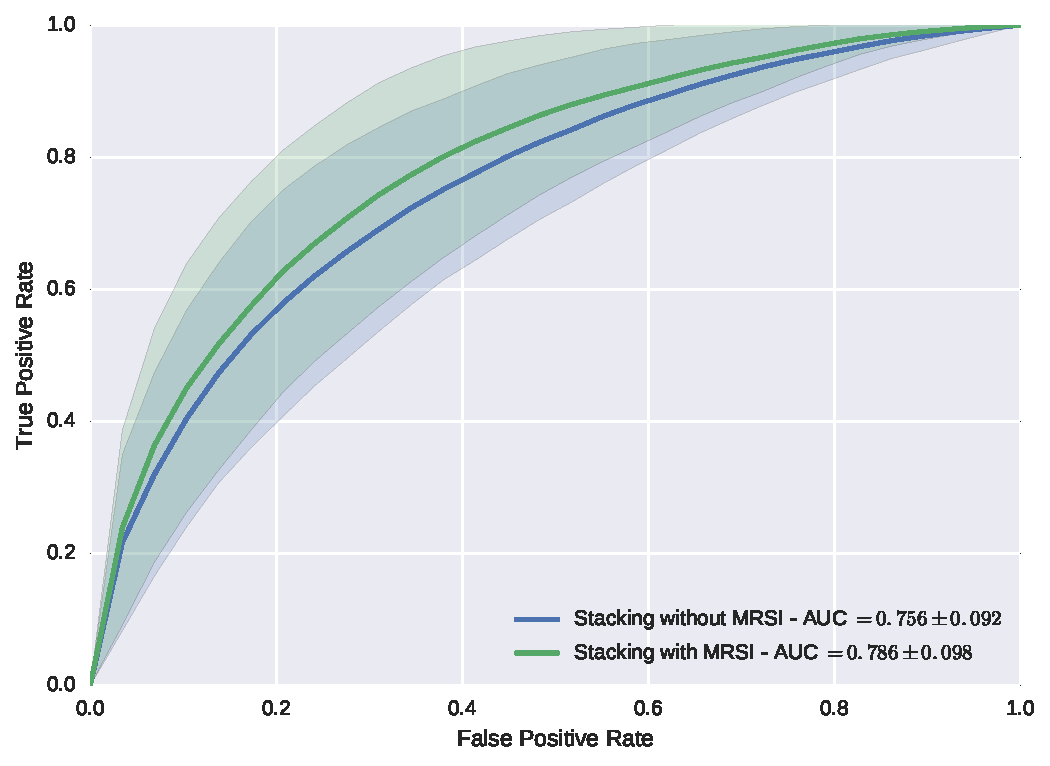
\includegraphics[width=0.7\linewidth]{content/figures/exp-6/stacking_wt_mrsi.pdf}
  \caption{Illustration of the gain of including the \acs*{mrsi} modality in a \acs*{mpmri} \acs*{cad}.}
  \label{fig:resmrsigain}
\end{figure}

We recall that the goal of this thesis is to use all the \ac{mpmri} modalities.
In this regard, \ac{mrsi} has nearly never been used together with the other modalities --- i.e., \ac{t2w}-\ac{mri}, \ac{dce}-\ac{mri}, and \ac{adc} map --- apart of the recent work of \citeauthor{trigui2017automatic}~\cite{trigui2016classification,trigui2017automatic}.
Therefore, we propose in this experiment to compare the classification performance by removing the \ac{mrsi} features.
In this regard, we propose to train 2 stacking classifiers --- with a \ac{gb} as meta-classifier --- while removing the feature related to \ac{mrsi} for one of them.
The same \ac{lopo} validation model is used as before and the results obtained from \ac{roc} analysis are depicted in \acs{fig}\,\ref{fig:resmrsigain}.

Therefore, including \ac{mrsi} into the classification pipeline increases the \ac{auc} from $0.756 \pm 0.092$ to $0.786 \pm 0.098$ for a gain of $0.030$.


\section{Discussion and conclusion}\label{sec:chp6:discussion}

We would like to stress the following findings drawn during the previous experiments.
The classification of individual modality highlights the weakness of the quantification methods --- i.e., pharmokinetic models, semi-quantitative model, and relative quantification of metabolites --- which might be due to the loss of information during the quantification procedure.
Furthermore, the features extracted from the \ac{t2w}-\ac{mri} are the most discriminative even after features selection.
Unlike \ac{t2w}-\ac{mri}, \ac{dce}-\ac{mri} is always the less efficient method.

The experiment link to the feature selection highlights some interesting facts regarding the most efficient features.
On the one hand, the Gabor filters and the phase congruency are always selected, independently of the strategy and modality during the feature selection process.
Additionally, edge filters --- i.e., Kirsch, Prewitt, Scharr, and Sobel --- have been only selected for the \ac{t2w}-\ac{mri}.
A possible explanation might be due to the fact that \ac{t2w}-\ac{mri} is the modality with the highest spatial resolution and in which the level of details is the most important.
Subsequently, the intensity feature of the \ac{t2w}-\ac{mri} modality is always selected, implying that our normalization method proposed in \acs{sec}\,\ref{sec:chp5:T2-norm} is efficient.

While applying the feature selection on the concatenated set of features, \ac{mrsi} appeared to be one of the most significant feature by keeping most of the information.
Along the same line, we show that removing this modality from the stacking classifier decreases drastically the classification performance.

Finally, we can highlight that the classification performance obtained are the worst with patients having a \ac{cap} localized in the \ac{cg}. 

As avenues for future research, one could switch from voxel-based classification to super-voxel classification such that spatial structure are classified instead of voxel.
Furthermore, all features from this chapter can be defined as hand-crafted features.
Therefore, an approach with unsupervised learning as convolutional neural network and conjunction with transfer learning should be investigated.

%%% Local Variables: 
%%% mode: latex
%%% TeX-master: "../thesis"
%%% End: 



Therefore, including \ac{mrsi} into the classification pipeline increases the \ac{auc} from $0.756 \pm 0.092$ to $0.786 \pm 0.098$ for a gain of $0.030$.

%%%%%%%%%%%%%%%%%%%% End comment



% \begin{table[bt]
% \caption{This is a table. Tables should be self-contained and complement, but not duplicate, information contained in the text. They should be not be provided as images. Legends should be concise but comprehensive – the table, legend and footnotes must be understandable without reference to the text. All abbreviations must be defined in footnotes.}
% \begin{threeparttable}
% \begin{tabular}{lccrr}
% \headrow
% \thead{Variables} & \thead{JKL ($\boldsymbol{n=30}$)} & \thead{Control ($\boldsymbol{n=40}$)} & \thead{MN} & \thead{$\boldsymbol t$ (68)}\\
% Age at testing & 38 & 58 & 504.48 & 58 ms\\
% Age at testing & 38 & 58 & 504.48 & 58 ms\\
% Age at testing & 38 & 58 & 504.48 & 58 ms\\
% Age at testing & 38 & 58 & 504.48 & 58 ms\\
% \hiderowcolors
% stop alternating row colors from here onwards\\
% Age at testing & 38 & 58 & 504.48 & 58 ms\\
% Age at testing & 38 & 58 & 504.48 & 58 ms\\
% \hline  % Please only put a hline at the end of the table
% \end{tabular}

% \begin{tablenotes}
% \item JKL, just keep laughing; MN, merry noise.
% \end{tablenotes}
% \end{threeparttable}
% \end{table}

% \section*{acknowledgements}
% Acknowledgements should include contributions from anyone who does not meet the criteria for authorship (for example, to recognize contributions from people who provided technical help, collation of data, writing assistance, acquisition of funding, or a department chairperson who provided general support), as well as any funding or other support information.

% \section*{conflict of interest}
% The authors report no potential conflicts of interest. 

% \printendnotes

% Submissions are not required to reflect the precise reference formatting of the journal (use of italics, bold etc.), however it is important that all key elements of each reference are included.
% \bibliography{sample}
\bibliography{literature_review_2}

\begin{biography}[example-image-1x1]{A.~One}
Please check with the journal's author guidelines whether author biographies are required. They are usually only included for review-type articles, and typically require photos and brief biographies (up to 75 words) for each author.
\bigskip
\bigskip
\end{biography}

\graphicalabstract{example-image-1x1}{Please check the journal's author guildines for whether a graphical abstract, key points, new findings, or other items are required for display in the Table of Contents.}

\end{document}
